\chapter{Fast Concurrent Data Sketches}
\label{chap:fast-concurrent-data-sketches}

Data sketches are approximate succinct summaries of long data streams. They are widely used
for processing massive amounts of data and answering statistical queries about it.
Existing libraries producing sketches are very fast, but do not allow parallelism for 
creating sketches using multiple threads or querying them while
they are being built. In this chapter, we present a generic approach to parallelizing data sketches efficiently and
allowing them to be queried in real time,
while bounding the error that such parallelism introduces. Utilizing relaxed semantics and 
the notion of strong linearizability we prove our algorithm's correctness and analyze the 
error it induces in some specific sketches.
Our implementation achieves high scalability while keeping the error small. We have contributed
one of our concurrent sketches to the open-source data sketches library.

\section{Introduction}

\paragraph{Motivation.}
% Sketches are widely used
Data sketching algorithms, or \emph{sketches} for short~\cite{Cormode:2017}, have become 
an indispensable tool for high-speed computations over massive datasets in recent years. 
Their applications include a variety of analytics and machine learning use cases, e.g., data aggregation~\cite{agarwal2013mergeable, KMV}, graph mining~\cite{Cohen:2014}, anomaly (e.g., intrusion) detection~\cite{yang2018elastic}, real-time data analytics~\cite{druid}, and online classification~\cite{Tai:2018}.
%For example, sketches are instrumental in big data analytics systems, which ingest vast amounts of multidimensional data, 
%preprocess it, and provide statistical insights (unique element counts, quantile values, etc.) within interactive user experience 
%constraints. 

% What are sketches
Sketches are designed for \emph{stream} settings in which each data item is only processed once. A common use case is data analytics, powered by analytics platforms like Druid~\cite{druid}. A typical stream processing pipeline for data analytics is illustrated in Figure~\ref{fc-fig:pipeline}. The stream consists of real-time events from various sources, such as web page clicks, apps being run on mobile devices, social media posts, and reports from IoT devices. The data is typically stored for archival purposes, and also summarized by data sketches to allow real-time queries. Another use case is network management~\cite{Cormode:2017}, where statistics are gathered over a stream of network packets.  

\begin{figure}[htb]
  \begin{subfigure}[b]{.45\linewidth}
      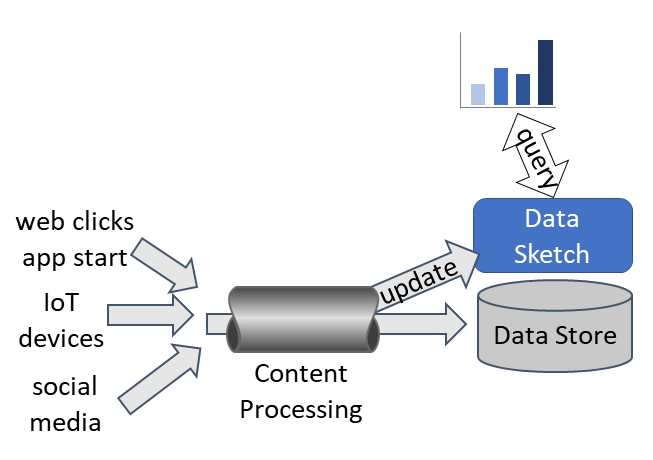
\includegraphics[height=1.6in]{graphics/fast-concurrent/pipeline-crop.png}
  \caption{Stream processing pipeline with data sketch.}
  \label{fc-fig:pipeline}
  \end{subfigure}
  \begin{subfigure}[b]{.55\linewidth}
    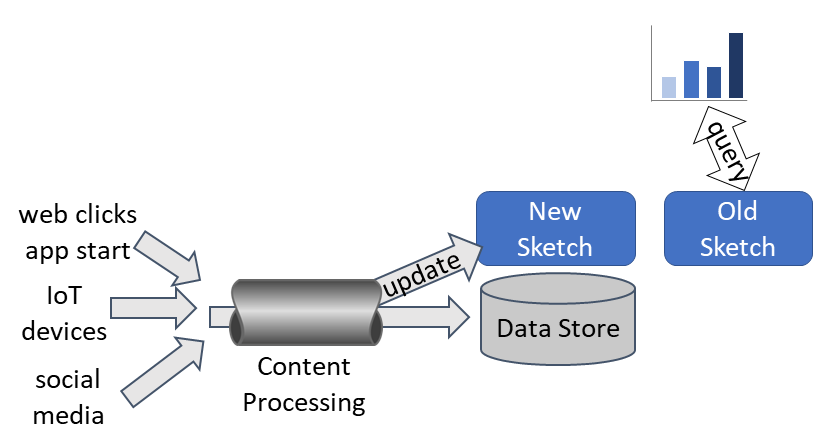
\includegraphics[height=1.6in]{graphics/fast-concurrent/epochs-crop.png}
  \caption{Using sketches in epochs.}
  \label{fc-fig:epochs}
  \end{subfigure}
\end{figure}

A sketch data structure is essentially a succinct (sublinear) summary of a stream that approximates a specific query, for instance, unique element count, quantile values, or frequent items. 
The approximation is typically very accurate -- the error drops fast with the stream size~\cite{Cormode:2017}. 

% Sketches today are sequential
Practical sketch implementations have recently emerged in toolkits~\cite{DataSketches}
and data analytics platforms (e.g., PowerDrill~\cite{heule2013hyperloglog}, Druid~\cite{druid}, 
Hillview~\cite{hillview}, and Presto~\cite{PrestoHLL}). 
However, these implementations are not thread-safe, allowing neither
parallel data ingestion nor concurrent queries and updates; concurrent use is prone to exceptions and 
gross estimation errors. Applications using these libraries are therefore required to explicitly protect all sketch API calls by locks~\cite{lee-groups-post, lee-issue}.
As a consequence of this limitation, typical deployments create sketches in epochs, where queries are referred to the sketch created in the previous epoch while new stream elements are directed to a new sketch, as illustrated in Figure~\ref{fc-fig:epochs}. This practice leads to stale query results and thus
loses the real-time quality of the system.  

\paragraph{Our approach.}
We present a generic approach to parallelizing data sketches efficiently while bounding the error that such a parallel implementation might induce. Our goal is to enable simultaneous queries and updates to the same sketch from multiple threads. Our solution is carefully designed to do so without slowing down operations as a result of synchronization.
This is particularly challenging because sketch libraries are extremely fast, often processing tens of millions of updates per second. 

We capitalize on the well-known sketch \emph{mergeability} property~\cite{Cormode:2017}, which enables computing a sketch 
over a stream by merging sketches over sub-streams. Previous works have exploited this property for distributed 
stream processing (e.g.,~\cite{heule2013hyperloglog, cormode2011algorithms}), devising solutions with a sequential bottleneck at the merge phase and where queries cannot
be served before all updates complete. 
In contrast, our method is based on shared memory and constantly propagates results to a queryable sketch.
Our solution architecture is illustrated in Figure~\ref{fc-fig:arch}. Multiple worker thread buffer updates in local sketches and periodically merge them into a global sketch; queries access the latter. 

\begin{figure}[htb]
  \begin{center}
    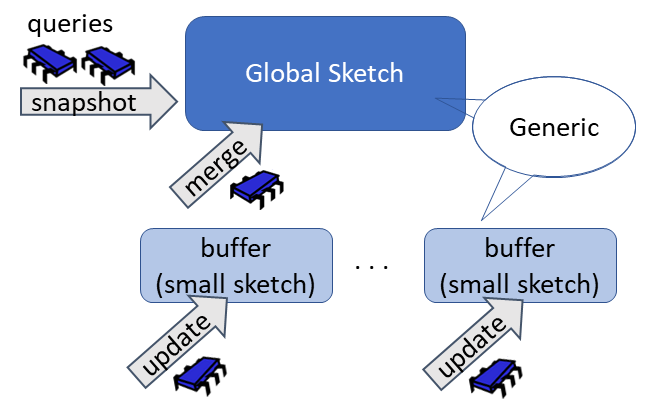
\includegraphics[width=0.5\textwidth]{graphics/fast-concurrent/arch-crop.png}
  \end{center}
  \caption{Concurrent sketches architecture.}
  \label{fc-fig:arch}
\end{figure}


We adaptively parallelize  stream processing:  
for small streams, we forgo parallel ingestion as it might introduce significant errors;  
but as the stream becomes large, we process it in parallel using small
thread-local sketches with continuous background propagation of local results to the common (queryable) sketch.

We instantiate our generic algorithm with a KMV $\Theta$ sketch~\cite{KMV},
which estimates the number of unique elements in a stream; a popular sketch
from the open-source Apache DataSketches library~\cite{DataSketches}.
We have contributed our implementation back to the Apache DataSketches 
library~\cite{ConcurrentThetaImp}. 
Yet we emphasize that our design is generic and applicable to additional sketches. 
We briefly discuss the applicability of our algorithm to additional popular sketches, such as Quantiles, CountMin, and HyperLogLog, 
where we discuss the generic algorithm (cf.~Section~\ref{fc-sec:genericAlg}).

Figure~\ref{fc-fig:performance} compares
the ingestion throughput of our concurrent $\Theta$ sketch to that of a lock-protected sequential sketch,
on multi-core hardware. As expected, the trivial solution does not scale whereas our algorithm scales linearly. 


\begin{figure}[htb]
  \begin{center}
    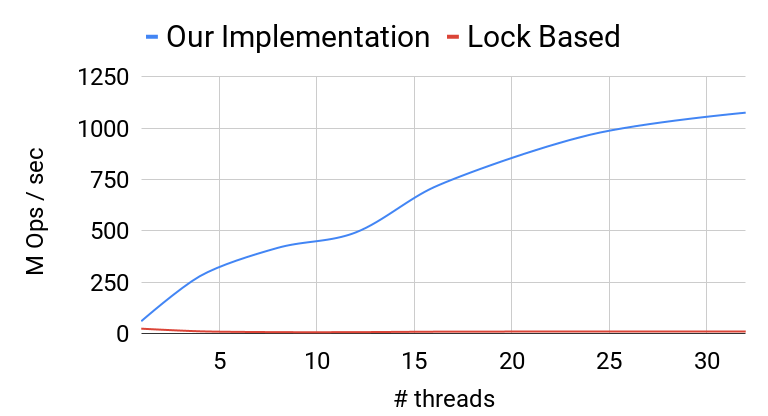
\includegraphics[width=0.6\textwidth]{graphics/fast-concurrent/concurrentThetaGraph.png}
  \end{center}
  \caption{Scalability of DataSketches' $\Theta$ sketch 
   protected by a lock vs.\ our concurrent implementation.}
  \label{fc-fig:performance}
\end{figure}

\paragraph{Error analysis.}
Concurrency might induce an error, and one of the main challenges we address is analyzing this error.
To begin with, our concurrent sketch is a concurrent data structure, and 
we need to specify its  semantics. We do so using a flavor of 
%\emph{relaxed consistency} due to Henzinger et al.~\cite{Henzinger}    
\emph{relaxed consistency} similar to~\cite{Henzinger, alistarh2018distributionally, talmage2014improving}    %specifically, a restricted form of their   \emph{out-of-order} relaxation 
that allows operations to ``overtake'' some other operations.  
Thus, a query may return a result that reflects all but a bounded number of the updates
that precede it. 
While relaxed semantics were previously used for data structures such as stacks~\cite{Henzinger}
and priority queues~\cite{alistarh, rihani2014multiqueues}, we believe that they are a natural fit for data sketches. 
This is because sketches are typically used to summarize streams that  arise from multiple real-world sources  
and are collected over a network with variable delays, and so even if the sketch ensures strict semantics, 
queries might miss some real-world events that occur before them. Additionally, sketches are inherently approximate.
Relaxing their semantics therefore ``makes sense'', as long as it does not excessively increase the expected error.
%Add that the error is addative and not multplicative
If a stream is much longer than the relaxation bound, then indeed the error induced by the relaxation is negligible. For instance, in a stream consisting of ten million events, missing a hundred (or even a thousand) of them will not make a big impact. 

Analytics platforms often use multiple sketches in order to capture different dimensions of the data. For instance, they may count the number of unique users from each region in a different sketch. 
Typically, a handful of popular sketches account for most events, and others are updated less frequently. Whereas the relaxation does not significantly affect the estimation in the popular sketches, since the error allowed by the relaxation is additive, in less popular sub-streams, it may have a large impact. 
This motivates our adaptive solution, which forgoes relaxing small streams altogether. 

% correctness roadmap: derandomise,  strong serialisability, Adversary model,

We show that under parallel ingestion, our algorithm satisfies relaxed consistency with a relaxation of up to $2Nb$, where $N$ is the number of worker threads and $b$ is the buffer size of each worker.  
In our example use case, $N$ is $12$ and $b$ ranges between $1$ and $5$. 

% But this raises a new difficulty: 
The proof involves some technical challenges. First, relaxed consistency is defined with regards to a deterministic specification, whereas sketches are randomized.
We therefore first de-randomize the sketch's behavior
by delegating the random coin flips to an oracle. We can then relax the resulting sequential specification.
Next, because our concurrent sketch is used within randomized algorithms, 
it is not enough to prove its linearizability. Rather, 
we prove that our generic concurrent algorithm instantiated with sequential sketch $S$
satisfies \emph{strong linearizability}~\cite{Wojciech} with regards to a relaxed sequential specification of the de-randomized $S$. We note, however, that supporting strong linearizability
did not incur additional costs nor did it impact the relaxation; we were able to prove that our original design was strongly linearizable. 

We then analyze the error for two types of relaxed sketches under random coin flips, with an adversarial scheduler that may delay operations in a way that maximizes the error. First, we consider the $\Theta$ sketch. For this sketch, its relative standard error has been analyzed, and we
show  that our concurrent implementation's error is coarsely bounded by twice
that of the corresponding sequential sketch. Second, we consider a family of \emph{probably approximately correct (PAC)}
sketches -- these are sketches that estimate some quantity with an error of at most $\epsilon$ with a probability of at least $1-\delta$. 
For an arbitrary PAC sketch estimating quantiles or counting unique elements, we show that the error induced by its relaxation approaches that of the original, non-relaxed sketch as the stream size tends to infinity.

\paragraph{Main contribution.} In summary, this paper tackles the problem of concurrent sketches,
offers a general efficient solution for it, and rigorously analyses this solution. While the
paper makes use of many known techniques, it combines them in a novel way.
The main technical challenges we address are (1) devising a high-performance generic algorithm 
that supports real-time queries concurrently with updates without inducing an excessive error; 
(2) proving the relaxed consistency of the algorithm; 
and (3) bounding the error induced by the relaxation in both short and long streams.

The paper proceeds as follows:
Section~\ref{fc-sec:model} lays out the model for our work and Section~\ref{fc-sec:background} provides background
on sequential sketches. In Section~\ref{fc-sec:concurrentSketches} we formulate a flavor of relaxed semantics
appropriate for data sketches. Section~\ref{fc-sec:genericAlg} presents our generic algorithm, and Section~\ref{fc-sec:proofs}
proves strong linearizability of our generic algorithm. Section~\ref{fc-sec:error-bounds} analyses
error bounds for example sketches. Section~\ref{fc-sec:eval} empirically studies the $\Theta$ sketch's performance
and error with different stream sizes. Finally, Section~\ref{fc-sec:discussion}
concludes.

\section{Model}
\label{fc-sec:model}

We consider a non-sequentially consistent shared memory model that enforces program order on all variables and allows explicit 
definition of \emph{atomic} variables as in Java~\cite{JavaMemoryModel} and C++~\cite{CppConcurrentMemoryModel}.
Practically speaking, reads and writes of atomic variables are guarded by memory fences, which guarantee
that all writes executed before a write {\sc w} to an atomic variable are visible to all
reads that follow (on any thread) a read {\sc r} of the same atomic variable s.t.\ {\sc r} occurs after {\sc w}. 


A thread takes \emph{steps} according to a deterministic \emph{algorithm} defined as a state machine, 
where a step can access a shared memory variable, do local computations, and possibly return some value.
%Every step is a 3-tuple  $\left\langle state, action, state' \right\rangle$ where \emph{action} is defined by the thread's state machine.
An \emph{execution} of an algorithm is an alternating sequence of steps and states, where  each step follows some thread's state machine.
Algorithms implement objects supporting \emph{operations}, such as query and update. 
An operation's execution consists of a series of steps, beginning with a special \emph{invoke} step and ending in a \emph{response}
step that may return a value. 
The \emph{history} of an execution $\sigma$, denoted ${\mathcal{H}}(\sigma)$, 
is its subsequence of operation invoke and response steps.
In a \emph{sequential history}, each invocation is immediately followed by its response.
The \emph{sequential specification (SeqSpec)} of an object is its set of allowed sequential histories.

%Correctness of concurrent algorithms is typically formulated using the notion of
%linearisability~\cite{herlihy1990linearizability}: 
A \emph{linearization} of a concurrent execution $\sigma$ is a history $H \in$\emph{SeqSpec}
such that (1) after adding responses to some pending invocations in $\sigma$ and removing others,
$H$ and $\sigma$ consist of the same invocations and responses (including parameters)
and (2) $H$ preserves the order between non-overlapping operations in $\sigma$.
Golab et al.~\cite{Wojciech} have shown that in order to ensure
correct behavior of randomized algorithms under concurrency,
one has to prove \emph{strong linearizability}:

\begin{definition}[Strong linearizability]
A function $f$ mapping executions to  histories is \emph{prefix preserving} if
for every  two executions $\sigma, \sigma'$ s.t.\ $\sigma$ is a prefix of $\sigma'$,  
$f(\sigma)$ is a prefix of $f(\sigma')$.

An algorithm $A$ is a strongly linearizable implementation of an 
object $o$ if there is a prefix preserving function $f$ that maps 
every execution $\sigma$ of $A$ to a linearization $H$ of $\sigma$.
\end{definition}

For example, executions of atomic variables are strongly linearizable.

\section{Background: sequential sketches}
\label{fc-sec:background}

A sketch $S$ summarizes a collection of elements $\Collection{a_1,a_2,\dots,a_n}$, processed
in some order given as a stream $A=a_1,a_2,\dots,a_n$.
The desired summary is agnostic to the processing order,
but the underlying data structures may differ due to the order. Its API is:

\begin{description}
\item[$S$.init()] initializes $S$ to summarize the empty stream;
\item[$S$.update($a$)] processes stream element $a$;
\item[$S$.query($arg$)] returns the function estimated by the sketch over the stream processed thus far, e.g., the number of unique elements; 
 takes an optional argument, e.g., the requested quantile.
 \item[$S$.merge($S'$)] merges sketches $S$ and $S'$ into $S$; i.e., if $S$ initially summarized stream $A$ and $S'$ 
 summarized $A'$, then after this call, $S$ summarizes the concatenation of the two, $A||A'$.
\end{description}

\paragraph{Example: $\Theta$ sketch.}

\begin{algorithm}[htb]
    \small
    %\begin{multicols}{2}
    \begin{algorithmic}[1]
        %\begin{varwidth}[t]{0.9\linewidth} 
        \Vars
        \State   sampleSet, init $k$ $1$'s \Comment samples
        \State  $\Theta$, init $1$			\Comment threshold
        \State {\tt atomic} est, init $0$ \Comment estimate
        \State $h$, init random uniform hash function 
        \EndFor
        
        \Procedure{query}{arg}
        \State \Return $est$ \label{fc-l:query}
        \EndProcedure
        
        \Procedure{update}{arg}
        \If{$h$(arg) $\geq \Theta$} \Return
        \EndIf
        \State add $h$(arg) to \emph{sampleSet}
        \State keep $k$ smallest samples in \emph{sampleSet}
        \State $\Theta \leftarrow max(sampleSet)$
        \State $\mathit{est}$ $\leftarrow $ $\left( |\text{sampleSet}|-1 \right)$ / $\Theta$
        \EndProcedure
        %\end{varwidth}\quad\quad\quad 
        %\columnbreak
        %\begin{varwidth}[t]{1\linewidth}

        \Procedure{merge}{S}
        \State sampleSet $\leftarrow$ merge sampleSet and $S$.sampleSet
        \State keep $k$ smallest values in sampleSet
        \State $\Theta \leftarrow max($sampleSet$)$
        \State $\mathit{est}$ $\leftarrow $ $\left( |\text{sampleSet}|-1 \right)$ / $\Theta$ \label{fc-l:update-est}
        \EndProcedure
        
    \end{algorithmic}
    %\end{multicols}
    \caption{$\Theta$ sketch.}
    \label{fc-alg:theta}
\end{algorithm}

Our running example is a $\Theta$ sketch based on the 
\emph{K Minimum Values (KMV)} algorithm~\cite{KMV} given in Algorithm~\ref{fc-alg:theta}. It maintains a \emph{sampleSet} and a parameter $\Theta$
that determines which elements are added to the sample set. 
It uses a random hash function $h$ whose outputs are uniformly distributed
in the range $[0,1]$, and $\Theta$ is always in the same range.  
An incoming stream element is first hashed, and then the hash is compared to $\Theta$. 
In case it is smaller, the value is added to \emph{sampleSet}.  Otherwise, it is ignored. 

Because the hash outputs are uniformly distributed, the expected proportion of values
smaller than $\Theta$ is $\Theta$. 
Therefore, we can estimate the number of unique elements in the stream by
dividing the number of (unique) stored samples by $\Theta$ (assuming that the random hash function is
drawn independently of the stream values).

KMV $\Theta$ sketches keep constant-size sample sets:
they take a parameter $k$ and keep the $k$ smallest hashes seen so far. 
$\Theta$ is $1$ during the first $k$ updates, and 
subsequently it is the hash of the largest sample in the set.
Once the sample set is full,
every update that inserts  a new element also removes the largest
one and updates $\Theta$. This is implemented efficiently using a min-heap.
The merge method adds a batch of samples to \emph{sampleSet}.

\paragraph{Accuracy.}

% Sequential specification
Today, sketches are used sequentially,
so that the entire stream is processed 
and then $S$.query(arg) returns an estimate of the desired function 
on the entire stream. Accuracy is defined in one of two ways.
One approach analyses the \emph{Relative Standard Error (RSE)} of the estimate, 
which is the standard error normalized by the quantity being estimated.
For example, a KMV $\Theta$ sketch with $k$ samples has an RSE of less than $1/\sqrt{k-2}$~\cite{KMV}.

 A PAC sketch provides a result that estimates the correct result
within some error bound $\epsilon$ with a failure probability bounded by some parameter $\delta$.  
For example, a Quantiles sketch approximates the $\phi$th quantile of a stream with $n$ elements 
by returning an element whose rank is in $\left[(\phi-\epsilon)n , (\phi+\epsilon)n \right]$ with 
probability at least $1-\delta$~\cite{agarwal2013mergeable}.

\section{Relaxed consistency for concurrent sketches}
\label{fc-sec:concurrentSketches}

Previous work by Alistarh et al.~\cite{alistarh2018distributionally} has presented a formalization for a randomized relaxation of an object.
The main idea is to have the parallel execution approximately simulate the object’s correct sequential behavior, with some provided error distribution.
In their framework, one considers the parallel algorithm and bounds the probability that it induces a large error
 relative to the deterministic sequential specification.
This approach is not suitable for our analysis, since the sequential object we parallelize (namely the sketch) is
itself randomized. Thus, there are two sources of error: (1) the approximation error in the sequential sketch and
(2) the additional error induced by the parallelization. For the former, we wish to leverage the
existing literature on analysis of sequential sketches. To bound the latter, we use a different
methodology: we first derandomize the sequential sketch by delegating its coin flips to an oracle,
and then analyze the relaxation of the (now) deterministic sketch. Finally, we leverage the sequential sketch
analysis to arrive at a distribution for the returned value of a query.


We adopt a variant of Henzinger et al.'s~\cite{Henzinger} {\emph{out-of-order}} relaxation,  
which generalizes quasi-linearizabilty~\cite{afek2010quasi}.
Intuitively, this relaxation allows a query to ``miss'' a bounded number of updates that precede it.
Because a sketch is order agnostic, we further allow re-ordering of the updates ``seen'' by a query.

\begin{definition}[r-relaxed history]
  A sequential history $H$ is an \emph{r-relaxation} of a sequential history $H'$,
  if $H$ is comprised of all but at most $r$ of the invocations in $H'$ and their responses,
  and each invocation in $H$ is preceded by all but at most $r$ of the invocations that precede the 
  same invocation in $H'$. 
\end{definition}

A relaxed property for an object $o$ is an extension of its sequential specification to include also
relaxed histories and thus allow more behaviors. This requires $o$ to have a sequential specification, so
we convert sketches into deterministic objects by capturing their randomness in an external oracle; 
given the oracle's output, the sketches behave deterministically.
For the $\Theta$ sketch, the oracle's output is passed as a hidden variable to $init$, where the sketch
selects the hash function. In the Quantiles sketch, a coin flip is provided with every update.

For a derandomized sketch, we refer to the set of histories arising in its sequential
executions as \emph{SeqSketch}, and use SeqSketch as its sequential specification.
We can now define our relaxed semantics:
\begin{definition}[r-relaxation]
The \emph{r-relaxation} of SeqSketch is the set of histories that have r-relaxations in SeqSketch:
  
\[ SeqSketch^r \triangleq \{H'|\exists H\in \textrm{SeqSketch s.t. H is an r-relaxation of}\ H'\}.\]

\label{fc-def:r-relaxtion}
\end{definition}

Note that our formalism slightly differs from that of~\cite{Henzinger} in that we start with a serialization $H'$ of an object’s
execution that does not meet the sequential specification and then ``fix'' it by relaxing it to a history $H$ in the sequential
specification. In other words, we relax history $H'$ by allowing up to $r$ updates to ``overtake'' every query, so the
resulting relaxation $H$ is in SeqSketch.
\begin{figure}[ht]
%\begin{wrapfigure}{r}{0.4\textwidth}
    \begin{center}
      %\vspace{-0.3in}
      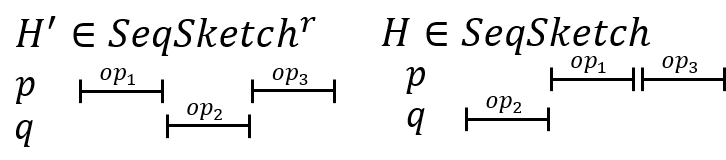
\includegraphics[width=0.5\textwidth]{graphics/fast-concurrent/relaxationExample}
      %\vspace{-0.3in}
    \end{center}
    \caption{$H$ is a 1-relaxation of $H'$.}
    \label{fc-fig:relaxationExample}
%\end{wrapfigure}
\end{figure}

An example is given in Figure~\ref{fc-fig:relaxationExample}, where $H$ is a 1-relaxation of history $H'$.
Both $H$ and $H'$ are sequential, as the operations don't overlap.
%In history $H$, $op_2$ has ``overtaken'' $op_1$ to appear first.

The impact of the $r$-relaxation on the sketch's error depends on the \emph{adversary}, which may select up to 
$r$ updates to hide from every query. There exist two adversary models:   
A \emph{weak adversary} decides which $r$ operations to omit from 
every query without observing the coin flips. 
A \emph{strong adversary} may select which updates to hide after learning 
the coin flips. Neither adversary sees the protocol's internal state, however both know the algorithm
and see the input. As the strong adversary knows the coin flips, it can then extrapolate the state; the
weak adversary, on the other hand, cannot.




\section{Generic concurrent sketch algorithm}
\label{fc-sec:genericAlg}

We now present our generic concurrent  algorithm. 
The algorithm uses, as a building block, an existing (non-parallel) sketch. 
To this end, we extend the standard sketch interface in Section~\ref{fc-sec:composable-sketches}, 
making it usable within our generic framework. That is, any sketch exposing this extended API can be used within our framework.
Our algorithm is adaptive -- it serializes ingestion in small streams and parallelizes it in large ones.
For clarity of presentation, we  present in Section~\ref{fc-sec:basic-generic-alg} the parallel phase of the algorithm,
which provides relaxed semantics appropriate for large streams.  
%in the full paper~\cite{rinberg2019fast}
%in Section~\ref{sec:proofs} we prove that it is strongly linearisable with respect to an $r$-relaxation of the sequential sketch with which it is instantiated.
Section~\ref{fc-ssec:small-streams} then discusses the adaptation for small streams.


\subsection{Composable sketches}
\label{fc-sec:composable-sketches}

In order to be able to build upon an existing sketch \emph{S},
we first extend it to support a limited form of concurrency.
Sketches that support this extension are called \emph{composable}.

A composable sketch has to allow concurrency between merges and queries.
To this end, we add a \emph{snapshot} API that can run concurrently with merge and
obtains a queryable copy of the sketch. The sequential specification of this operation is as follows:
\begin{description}
    \item[$S$.snapshot()] returns a copy $S'$ of $S$ such that immediately after $S'$ is returned,
     $S$.query($arg$) = $S'$.query($arg$) for every possible $arg$.
\end{description}

A composable sketch needs to allow concurrency only between snapshots
and other snapshot and merge operations. In general, we require that such concurrent
executions be strongly linearizable. Our $\Theta$ sketch, shown below,
simply accesses an atomic variable that holds the query result. In other sketches, for instance, 
CountMin~\cite{CountMin}, HyperLogLog~\cite{Flajolet07hyperloglog,heule2013hyperloglog,druid,PrestoHLL}, and Quantiles~\cite{KLL:2016}, atomic
snapshots can be achieved in a straightforward manner via a double collect of the relevant state, e.g., array of counters.
In specific sketches, this may be optimized in different ways. 

In recent work~\cite{rinberg_et_al:LIPIcs:2020:13080}, we have shown that for PAC objects, a linearizable snapshot is often not necessary for preserving the sketch's error bounds. We defined a relaxation of linearizability, called \emph{Intermediate Value Linearizability (IVL)}. We proved that for any sequential PAC object  -- that is, one guaranteeing an error of at most $\epsilon$ with a probability of at least $1-\delta$ for some parameters $\epsilon$ and $\delta$ -- any concurrent implementation of this object that satisfies IVL guarantees the same $\epsilon, \delta$ error bounds as the sequential object. In many cases, this allows replacing the linearizable snapshot with a single collect of the data structure, which is an array of counters in sketches like CountMin and HyperLogLog. In such cases, the implementation of the snapshot function is identical to the sequential sketch's query operation, and no synchronization is required. 

\paragraph{Pre-filtering.} When multiple sketches are used in a multi-threaded algorithm,
we can optimize them by sharing ``hints'' about the processed data.
This is useful when the stream sketching function depends on the processed stream prefix.
For example, we explain below how $\Theta$ sketches sharing a common value of $\Theta$ can sample fewer updates.
Another example is reservoir sampling~\cite{vitter1985random}. To support this optimization,
we add the following two APIs:
\begin{description}
    \item[$S$.calcHint()] returns a value $h \neq 0$ to be used as a hint.
    \item[$S$.shouldAdd($h$, $a$)] given a hint $h$ and a stream element $a$, returns a Boolean indicating whether $a$
		should be added to the sketch, or may be filtered out as it does not affect the sketch's state.
\end{description}    
%    Note that $S$.shouldAdd is a static function that does not depend on the current state of $S$.
    Formally, the semantics of these APIs are defined using the notion of summary.
		(1) Consider a sketch $S$ initialized in some state $s_0$. We say that $s_0$ (or the sketch at time $0$) \emph{summarizes} the empty history,
    and similarly, the empty stream; we refer to the sketch as \emph{empty}.
		(2) Let $s'$ be the sketch's state after we sequentially ingest a stream $a_1, \dots ,a_n$, namely after 		
		a sequential execution with the history 
		\[H= S.update(a_1), S.resp, \dots S.update(a_n), S.resp.\] 
		We say that $s'$ \emph{summarizes} history $H$, and,
    similarly, summarizes the stream $a_1, \dots ,a_n$.
    
		Given a sketch state $s'$ that summarizes a stream $A$, if shouldAdd($S.calcHint()$, $a$) returns false then
    for every streams $B_1,B_2$ and sketch state $s'$ that summarizes $A||B_1||a||B_2$,
    $s'$ also summarizes $A||B_1||B_2$. Note that a state summarizes two different streams if and only if that state is reached
		after ingesting each of them to an empty sketch.

These APIs do not need to support concurrency, and may be trivially implemented by always returning $true$.
Thus, they do not impose additional constraints on the set of sketches usable with our generic algorithm.


\paragraph{Example: composable $\Theta$ sketch.}
 
Algorithm~\ref{fc-alg:composable-theta} presents the three additional APIs for the $\Theta$ sketch.
The composable sketch is used concurrently by a single updater thread and multiple query threads. 
The \emph{est} variable is atomic, and is shared among all threads; the remaining state variables are local to the updating thread.

The snapshot method copies $\mathit{est}$. Note that the
result of a merge is only visible after writing to est, because it is the only variable accessed by
the query. As \emph{est} is an atomic variable, the requirement on snapshot and merge is
met. To minimize the number of updates, calcHint returns $\Theta$
and shouldAdd checks if $h(a) < \Theta$, which is safe because the value of
$\Theta$ in sketch $S$ is monotonically decreasing. Therefore, if $h(a) \geq \Theta$
then $h(a)$ will never enter the \emph{sampleSet}.

\begin{algorithm}[htb]
    \small
    %\begin{multicols}{2}
    \begin{algorithmic}[1]
       
        \Procedure{snapshot}{}
            \State $localCopy \leftarrow empty sketch$
            \State $localCopy.\mathit{est} \leftarrow \mathit{est}$
            \State \Return $localCopy$
        \EndProcedure
    
        \Procedure{calcHint}{}
            \State \Return $\Theta$
        \EndProcedure
    
        \Procedure{shouldAdd}{H, arg}
            \State \Return $h$(arg) $< H$
        \EndProcedure
    %\end{varwidth}

    \end{algorithmic}
    %\end{multicols}
    \caption{Additional methods for composable $\Theta$ sketch.}
    \label{fc-alg:composable-theta}
\end{algorithm}

\subsection{Generic algorithm}
\label{fc-sec:basic-generic-alg}

We now present a generic concurrent sketch algorithm that can be instantiated with any composobale sketch adhering to the API defined in the previous section. To simplify the presentation, we first discuss an unoptimized version of
our generic concurrent algorithm, (left column in of Algorithm~\ref{fc-alg:generic-concurrent}),  called 
\emph{ParSketch}, and later an optimized version of the same algorithm (right column of Algorithm~\ref{fc-alg:generic-concurrent}).

The algorithm is instantiated by a composable sketch and sequential sketches.
It uses multiple threads to process incoming stream elements 
and services queries at any time during the sketch's construction.
Specifically, it uses $N$ worker threads, $t_1,\dots,t_N$, each of which samples
stream elements into a local sketch $localS_i$, and a propagator thread $t_0$ that merges local sketches
into a shared composable sketch $globalS$. Although the local sketch resides in
shared memory, it is updated exclusively by its owner update thread $t_i$ and 
read exclusively by $t_0$. Moreover, updates and reads do not happen in
parallel, and so cache invalidations are minimized. The global sketch is updated only by $t_0$
and read by query threads. We allow an unbounded number of query threads. 

After $b$ updates are added to $localS_i$, $t_i$ signals to the propagator to merge
it with the shared sketch. It synchronizes with $t_0$ using a 
single \emph{atomic} variable $prop_i$, which $t_i$ sets to 0.  
Because $prop_i$ is atomic, the memory model
guarantees that all preceding updates to $t_i$'s local sketch are visible to
the background thread once $prop_i$'s update is.
This signalling is relatively expensive (involving a memory fence),  
but we do it only once per $b$ items retained in the local sketch.

After signalling to $t_0$, $t_i$ waits
until $prop_i \neq 0$  (line~\ref{fc-l:wait}); 
this indicates that the propagation has completed, and $t_i$ can 
reuse its local sketch. Thread $t_0$ piggybacks the hint \emph{H} it
obtains from the global sketch on $prop_i$,
and so there is no need for further synchronization in order to pass the hint.

Before updating the local sketch, $t_i$ invokes shouldAdd to check
whether it needs to process \emph{a} or not. For example, the $\Theta$ sketch discards updates whose hashes are
greater than the current value of $\Theta$. The global thread passes the global sketch's
value of $\Theta$ to the update threads, pruning updates that would end up being discarded
during propagation. This significantly
reduces the frequency of propagations and associated memory fences.

\begin{algorithm}[htb]
    \footnotesize
   \begin{multicols}{2}
    \begin{algorithmic}[1]
    \setcounter{ALG@line}{100}

     \Statex {\bf Basic algorithm } 
    \Vars
    \State composable sketch \emph{globalS}, init empty
    \State constant $b$ \Comment relaxation is $2Nb$
    \ForEach{update thread $t_i$} , $0 \leq i \leq N$
        \State sketch \emph{localS$_i$}, init empty
	\State
        \State int $counter_i$, init $0$
        \State int \emph{hint}$_i$, init $1$
        \State int {\tt atomic} $prop_i$, init $1$
    \EndFor
    \EndFor

    \Procedure{propagator}{}
    \While {true}
    \ForAll{thread $t_i$ s.t. $prop_i=0$}
        \State $globalS.merge(localS_i)$ \label{fc-l:merge}
        \State $localS_i  \leftarrow $empty sketch \label{fc-l:emptyAux}
		\State $prop_i \leftarrow globalS.calcHint()$ \label{fc-l:calcHint}
    \EndFor
    \EndWhile
    \EndProcedure

   

    \Procedure{query}{arg}
    \State $localCopy \leftarrow globalS.snapshot(localCopy)$
    \State \Return $localCopy.query(arg)$
    \EndProcedure
    
    \Procedure{update$_i$}{$a$}
    \If{$\neg$shouldAdd(\emph{hint}$_i$, $a$)} \Return \label{fc-l:shouldAdd}
    \EndIf
    \State $counter_i \leftarrow counter_i + 1$ \label{fc-l:countup}
    \State $localS_i.update(a)$ \label{fc-l:update}
    \If{$counter_i = b$} \label{fc-l:checkfull}
    \State {$prop_i \leftarrow 0$} \label{fc-l:signal}
    \State wait until $prop_i \neq 0$ \label{fc-l:wait}
     \State
    \State \emph{hint}$_i \leftarrow prop_i$ \label{fc-l:updateHint}
    \State $counter_i \leftarrow 0$ \label{fc-l:zeroCounter}
    \State
    \EndIf
    \EndProcedure

\columnbreak
    \setcounter{ALG@line}{200}
    \Statex {\bf Optimised algorithm } 
    \Vars
    \State composable sketch \emph{globalS}, init empty
    \State constant $b$ \Comment relaxation is $2Nb$
    \ForEach{update thread $t_i$} , $0 \leq i \leq N$
        \State sketch \emph{localS$_i$}[$2$], init empty
        \State int \emph{cur}$_i$, init 0
        \State int $counter_i$, init $0$
        \State int \emph{hint}$_i$, init $1$
        \State int {\tt atomic} $prop_i$, init $1$
    \EndFor
    \EndFor

    \Procedure{propagator}{}
    \While {true}
    \ForAll{thread $t_i$ s.t. $prop_i=0$}
        \State $globalS.merge(localS_i$[1-$cur_i$]$)$ 
        \State $localS_i[1-cur_i] \leftarrow $empty sketch 
		\State $prop_i \leftarrow globalS.calcHint()$ 
    \EndFor
    \EndWhile
    \EndProcedure
   
    \Procedure{query}{arg}
    \State $localCopy \leftarrow globalS.snapshot(localCopy)$
    \State \Return $localCopy.query(arg)$
    \EndProcedure
    
    \Procedure{update$_i$}{$a$}
    \If{$\neg$shouldAdd(\emph{hint}$_i$, $a$)} \Return 
    \EndIf
    \State $counter_i \leftarrow counter_i + 1$ 
    \State $localS_i$[$cur_i$]$.update(a)$ \label{fc-opt:l:update}
    \If{$counter_i = b$} \label{fc-opt:l:checkfull}
    \State 
    \State wait until $prop_i \neq 0$  \label{fc-opt:l:wait}
    \State $cur_i \leftarrow 1 - cur_i$ \label{fc-opt:l:swap-local-aux}
    \State \emph{hint}$_i \leftarrow prop_i$ \label{fc-opt:l:updateHint}
    \State $counter_i \leftarrow 0$ \label{fc-opt:l:zeroCounter}


    \State $prop_i \leftarrow 0$ \label{fc-opt:l:signal}
    \EndIf
    \EndProcedure


    \end{algorithmic}
   \end{multicols}
    \caption{Generic concurrent algorithm.}
    \label{fc-alg:generic-concurrent}
\end{algorithm}



Query threads use the snapshot method, which can be safely run concurrently with merge,
hence there is no need to synchronize between the query threads and $t_0$. The freshness
of the query is governed by the $r$-relaxation.
%In the full paper~\cite{rinberg2019fast},
In Section~\ref{fc-subsec:Generic-algorithm-proof}
we prove Lemma~\ref{fc-lemma:genereic-strong} below, asserting that
the relaxation is $Nb$. This may seem straightforward as $Nb$ is the combined size of the
local sketches. Nevertheless, proving this is not trivial because the local sketches pre-filter
many additional updates, which, as noted above, is instrumental for performance. 

\begin{lemma}
    $ParSketch$ instantiated with $SeqSketch$ is strongly linearisable with regards to  \emph{SeqSketch}$^r$, where
		$r=2Nb$.
    \label{fc-lemma:genereic-strong}
\end{lemma}


A limitation of \emph{ParSketch} is that update threads are idle while waiting for the propagator to execute the merge. This
may be inefficient, especially if a single propagator iterates through many local sketches.
In the right column of Algorithm~\ref{fc-alg:generic-concurrent}, we  present
the optimized \emph{OptParSketch} algorithm, which improves thread utilization via
double buffering.

In \emph{OptParSketch}, $localS_i$ is an array of two sketches. When $t_i$ is ready to propogate $localS_i[cur_i]$, it
flips the $cur_i$ bit denoting which sketch it is currently working on (line~\ref{fc-opt:l:swap-local-aux}), 
and immediately sets $prop_i$ to 0 (line~\ref{fc-opt:l:signal}) in order to allow the propagator to
take the information from the other one. It then starts digesting updates in a fresh sketch.

Of course, the optimization is only useful as long as the propagator thread is fast enough to empty the 
inactive buffers before the active ones fill up. The number of threads where this will saturate is highly sketch-dependant. 
In the example of the $\Theta$ sketch, thanks to pre-filtering, the working threads filter out many updates without filling their buffers, so
merges are required infrequently, and we can scale to a large number of threads with a single propagator regardless of the buffer size. In sketches without pre-filtering, the scalability typically depends on the buffer size.

In Section~\ref{fc-subsec:Optimised-algorithm-proof}
we prove the correctness of the optimized
algorithm by simulating $N$ threads of \emph{OptParSketch}
using $2N$ threads running \emph{ParSketch}. We do this by showing
a \emph{simulation relation}~\cite{lynch1996distributed}. We use forward simulation (with
no prophecy variables), ensuring strong linearizability. We conclude the following theorem:
\begin{restatable}{rthm}{optgenereicstrong}
    \emph{OptParSketch} instantiated with $SeqSketch$ is strongly linearizable with regards to \emph{SeqSketch}$^r$, where
		$r=2Nb$.
    \label{fc-lemma:opt-genereic-strong}
\end{restatable}


\subsection{Adapting to small streams}
\label{fc-ssec:small-streams}

By Theorem~\ref{fc-lemma:opt-genereic-strong}, a query can miss up to $r$ updates. For small
streams, the error induced by this can be very large.
For example, the sequential $\Theta$ sketch answers queries with perfect accuracy in streams with
up to $k$ unique elements, but if $k<r$, the relaxation can miss \emph{all} updates.
In other words, while the additive error is guaranteed to be bounded by $r$, the relative 
error can be infinite.  

To rectify this, we implement \emph{eager propagation} for small streams, 
whereby update threads propagate updates immediately to the shared sketch 
instead of buffering them. 
% and the shared sketch is accessed sequentially (protected by a lock or CAS).  
Note that during the eager phase, updates are processed sequentially. 
Support for eager propagation can be added to Algorithm~\ref{fc-alg:generic-concurrent} 
by initializing $b$ to $1$ and having the propagator thread raise it to the
desired buffer size once the stream exceeds some pre-defined length. 
The correctness of the adaptation is straightforward, since the buffer size is only used locally and only impacts the relaxation.
The error analysis of the next section can be used to determine the adaptation point.


\section{Proofs}
\label{fc-sec:proofs}

In Section~\ref{fc-sec:analysis:definitions} we introduce some formalisms.
In Section~\ref{fc-subsec:Generic-algorithm-proof} we prove that
the unoptimized algorithm is strongly linearizable with respect to
the relaxed specification $SeqSketch^r$ with $r=Nb$. Finally,
in Section~\ref{fc-subsec:Optimised-algorithm-proof} we show that
the the optimized algorithm is strongly linearizable with respect to
the relaxed specification $SeqSketch^r$ with $r=2Nb$.

\subsection{Definitions}
\label{fc-sec:analysis:definitions}
Note that the only methods invoked by $ParSketch$ on $globalS$ are snapshot and merge, and since merge is
only invoked by $t_0$, the only concurrency is between a snapshot and another operation (snapshot or merge).
Recall that we required such executions of a composable sketch to be strongly linearizable. By slight abuse
of terminology, we refer to these operations as atomic steps, for example, we refer to the linearization
point of $globalS$.merge simply as ``$globalS$.merge step''.

Likewise, as $localS_i$ is only accessed sequentially by a
single thread, either $t_i$ or $t_0$ (using $prop_i$ to synchronize),
we refer to the method calls shouldAdd and update as atomic steps.

Because we prove only safety properties, we restrict out attention to finite executions.
For analysis purposes we use auxiliary counters:
\begin{itemize}
    \item An array $sig\_ctr[N]$, that counts the number of times each thread $t_i$ signals to the propagator (line~\ref{fc-l:signal}).
    \item An array $merge\_ctr[N]$ counting the number of times $t_0$ executes a merge with thread $t_i$'s local sketch (line~\ref{fc-l:merge}).
\end{itemize}

Recall that in Section~\ref{fc-sec:background}, we said that a sketch's state \emph{summarizes} a
stream or a sequential history if it is the state of a sketch that has processed
the stream or history. We now overload the term ``summarizes'' to apply also to threads.
\begin{definition}[Thread summary]
    Consider a time $t$ in an execution $\sigma$ of Algorithm~\ref{fc-alg:generic-concurrent}. If at time $t$ either $prop_i \neq 0$
    or $sig\_ctr[i]>merge\_ctr[i]$, then we say that update thread $t_i$ \emph{summarizes} the history
    summarized by $localS_i$ at time $t$. Otherwise, thread $t_i$ summarizes the empty history at time $t$.
    The propagator thread $t_0$ summarizes the same history as $globalS$ at any time during an execution $\sigma$.
\label{fc-def:thread-summary}
\end{definition}
Note that if the first condition ($prop_i \neq 0$ or $sig\_ctr[i]>merge\_ctr[i]$) is not satisfied,
this means that the propagator thread might be in the process of clearing $localS_i$ in line~\ref{fc-l:emptyAux}.


As we want to analyze each thread's steps in an execution, we first define the projection from
execution $\sigma$ onto a thread $t_i$.
\begin{definition}[Projection]
    Given a finite execution $\sigma$ and a thread $t_i$, $\sigma\Bigr|_{t_i}$ is the subsequence of
    $\sigma$ consisting of steps taken by $t_i$.
\end{definition}

We want to prove that each thread's summary corresponds to the sequence of updates
processed by that thread since the last propagation, taking
into account only those that alter local state variables. These are updates for which \emph{shouldAdd} returns
true.
\begin{definition}[Unpropogated updates]
    Given a finite execution $\sigma$, we denote by suff$_i(\sigma)$ the suffix of $\sigma \Bigr|_{t_i}$ starting 
    at the last $globalS$.merge($localS_i$) event, or the beginning of $\sigma$ if no such event exists. 
    The unpropogated suffix up\_suff$_i(\sigma)$ of update thread $i$ is 
    the subsequence of $\mathcal{H} ($suff$_i(\sigma))$ consisting of $update(a)$ executions in suff$_i(\sigma)$ for which
    shouldAdd$(hint_i, arg)$ returns true in line \ref{fc-l:shouldAdd}.
    \label{fc-def:unpropogated-suffix}
\end{definition}

We define the relation between a sequential history $H$ and a stream $A$.
\begin{definition}
    Given a finite sequential history $H$, ${\mathcal{S}}(H)$ is the stream $a_1,\dots,a_n$ such that $a_k$
    is the argument of the $k$th update in $H$.
\end{definition}

Finally, we define the notion of \emph{happens before} in a sequential history $H$.
\begin{definition}
    Given a finite sequential history $H$ and two method invocations $M_1,M_2$ in $H$, we denote $M_1 \prec_H M_2$
    if $M_1$ precedes $M_2$ in $H$.
\end{definition}

\subsection{Unoptimized algorithm proof} 
\label{fc-subsec:Generic-algorithm-proof}

Our strong linearizability proof uses two mappings, $f$ and $l$, from 
executions to sequential histories defined as follows.
For an execution $\sigma$ of $ParSketch$, we define a mapping $f$ 
by ordering operations according to \emph{visibility points} defined as follows: 
\begin{itemize}
\item
For a query, the visibility point is the snapshot operation it executes.
\item 
For an update$_i$($a$) where shouldAdd($prop_i$, $a$) returns false at time $t$, its visibility point is $t$.
\item
Otherwise, for an update$_i$($a$), let $t$ be the first time after its invocation in $\sigma$
when thread $i$ changes $prop_i$ to 0 (line~\ref{fc-l:signal}).
Its visibility point is the (linearization point of the) first merge that occurs with $localS_i$ after time t.
If there is no such time, then update$_i$($a$) does not have a visibility point, i.e., is not included in $f(\sigma)$
\end{itemize}
Note that in the latter case,
the visibility point may occur after the update returns, and so $f$ does not 
necessarily preserve real-time order. 
 
We also define a mapping $l$ by ordering operations according to
\emph{linearization points} defined as follows:
\begin{itemize}
    \item
    An updates' linearization point is its invocation
    \item
    A query's linearization point is its visibility point.
\end{itemize}
By definition, $l(\sigma)$ is prefix-preserving.

We show that for every execution $\sigma$ of $ParSketch$,
(1) $f(\sigma) \in SeqSketch$, and 
(2) $f(\sigma)$ is an $r$-relaxation of $l(\sigma)$ for $r=N b$.  
Together, this implies that $l(\sigma) \in SeqSketch^r$, as needed.

We first show that $Prop_i \neq 0$ if $t_i$'s program counter is not on lines \ref{fc-l:signal} or \ref{fc-l:wait}.
\begin{invariant}
    At any time during a finite execution $\sigma$ of $ParSketch$ for every $i=1,\dots,N$, if $t_i$'s program
    counter isn't on lines \ref{fc-l:signal} or \ref{fc-l:wait}, then $prop_i \neq 0$.
    \label{fc-inv:prop-neq-0}
\end{invariant}
\begin{proof}
    The proof is derived immediately from the algorithm: $prop_i$ is initialized to 1 and gets
    the value of 0 on line \ref{fc-l:signal}, and then waits on line \ref{fc-l:wait} until $prop_i \neq 0$.
    After continuing passed line \ref{fc-l:wait}, $prop_i \neq 0$ again.
\end{proof}

We also observe the following:
\begin{observation}
    Given a finite execution $\sigma$ of $ParSketch$, for every $i=1,\dots,N$, every execution
    of $globalS.merge(localS_i)$ in $\sigma$ (line~\ref{fc-l:merge}) is preceded by an execution of $prop_i \leftarrow 0$
    (line~\ref{fc-l:signal}).
\end{observation}

We observe the following relationship between $t_i$'s program counter and $sig\_ctr[i]$ and \linebreak
$merge\_ctr[i]$:
\begin{observation}
    At all times during a finite execution $\sigma$ of $ParSketch$, for every
    $i=1,\dots,N$, $merge\_ctr[i] \leq sig\_ctr[i] \leq merge\_ctr[i] + 1$.
    Moreover, if $t_i$'s program counter isn't on lines \ref{fc-l:signal} or \ref{fc-l:wait}, then $sig\_ctr[i]=merge\_ctr[i]$.
    \label{fc-obs:counter_relationship}
\end{observation}

We show that at every point in an execution, update thread $t_i$ summarizes up\_suff$_i(\sigma)$. 
In essence, this means that we have not ``forgotten" any updates.
\begin{invariant}
    At all times during a finite execution $\sigma$ of $ParSketch$, for every $i=1,\dots,N$, $t_i$ summarizes up\_suff$_i(\sigma)$.
    \label{fc-inv:update-thread-summary}
\end{invariant}
\begin{proof}
    The proof is by induction on the length of $\sigma$. The base is immediate.
    Next we consider a step in $\sigma$ that can alter the invariant. We assume the invariant is correct
    for $\sigma'$, and prove correctness for $\sigma=\sigma',step$. We consider only steps that
    can alter the invariant, meaning the step can 
    either lead to a change in up\_suff$_i(\sigma)$, or a change in the history summarized by $t_i$. This
    means we need to consider only 4 cases:
    \begin{itemize}

        \item A step $localS_i.update(arg)$ (line~\ref{fc-l:update}) by thread $t_i$.

        In this case, up\_suff$_i(\sigma)=$up\_suff$_i(\sigma'),update(arg)$.
        By the inductive hypothesis, before the step $localS_i$ summarizes up\_suff$_i(\sigma')$,
        and so after the update, $localS_i$ summarizes $\text{up\_suff}_i(\sigma'),$ \linebreak $update(arg)=\text{up\_suff}_i(\sigma)$.
        From Invariant~\ref{fc-inv:prop-neq-0} $prop_i \neq 0$, therefore, by Definition \ref{fc-def:thread-summary}, $t_i$ summarizes
        the same history as $localS_i$,
        i.e., up\_suff$_i(\sigma)$, preserving the invariant.

        \item A step $prop_i \leftarrow 0$ (line~\ref{fc-l:signal}) by thread $t_i$.
        
        By the inductive hypothesis, before the step, $t_i$ summarizes the 
        history up\_suff$_i(\sigma')$. Because before the step  $prop_i \ne 0$, $localS_i$ 
				summarizes the same history.
        As no update occurs, up\_suff$_i(\sigma')$=up\_suff$_i(\sigma)$. The step
        doesn't alter $localS_i$, so after the step, $localS_i$ still summarizes
        up\_suff$_i(\sigma)$. On this step the counter $sig\_ctr[i]$ is increased but $merge\_ctr[i]$
        is not, so $sig\_ctr[i]>merge\_ctr[i]$.
        Therefore, by Definition \ref{fc-def:thread-summary}, $t_i$ summarizes the same history as $localS_i$,
        namely up\_suff$_i(\sigma)$, preserving the invariant.

        \item A step $globalS.merge(localS_i)$ (line~\ref{fc-l:merge}) by thread $t_0$.
        
        By Definition~\ref{fc-def:unpropogated-suffix}, after this step up\_suff$_i(\sigma)$ is empty. As
        this step is a $merge$, $merge\_ctr[i]$ is increased by one, so $sig\_ctr[i]=merge\_ctr[i]$ by
        Observation~\ref{fc-obs:counter_relationship}.
        Therefore, by Definition \ref{fc-def:thread-summary}, $t_i$
        summarizes the empty history, preserving the invariant.

        \item A step $prop_i \leftarrow globalS.calcHint()$ (line~\ref{fc-l:calcHint}) by thread $t_0$
        
        Before executing the step, $t_0$ executed line~\ref{fc-l:emptyAux}. Thread $t_i$ is waiting
        for $prop_i \neq 0$ on line~\ref{fc-l:wait}, therefore has not updated $localS_i$.
        Therefore, by Definition~\ref{fc-def:thread-summary}, $localS_i$ summarizes the empty history.
        As a merge with thread $i$ was executed and no updates have been invoked, up\_suff$_i(\sigma)$
        is the empty history.
        The function $calcHint$ cannot return $0$, therefore after that step $prop_i \neq 0$.
        By Definition \ref{fc-def:thread-summary}, $t_i$ summarizes the same history as $localS_i$, i.e., the empty history.
        Therefore, $t_i$ summarizes up\_suff$_i(\sigma)$, preserving the invariant.
    \end{itemize}
\end{proof}

Next, we prove that $t_0$ summarizes $f(\sigma)$.
\begin{invariant}[History of propagator thread]
    Given a finite execution $\sigma$ of $ParSketch$, $t_0$ summarizes $f(\sigma)$.
    \label{fc-inv:G-partial-summary}
\end{invariant}
\begin{proof}
    The proof is by induction on the length of $\sigma$. The base is immediate.
    We assume the invariant is correct for $\sigma'$, and prove correctness for $\sigma=\sigma',step$.
    There are two steps that can alter the invariant.
    \begin{itemize}
        \item A step $globalS.merge(localS_i)$ (line~\ref{fc-l:merge}) by thread $t_0$.
        
        By the inductive hypothesis, before the step, $t_0$ summarizes $f(\sigma')$. And by
        Invariant~\ref{fc-inv:update-thread-summary}, before the update, $t_i$ summarizes
        up\_suff$_i(\sigma')$, and by Invariant~\ref{fc-inv:prop-neq-0} $localS_i$ summarizes the same history.
        Let $A={\mathcal{S}}(f(\sigma))$, and $B={\mathcal{S}}($up\_suff$_i(\sigma')$$)$.
        After the merge $globalS$ summarizes $A||B$. Therefore,
        $t_0$ summarizes $f(\sigma)$ preserving the invariant.

        \item A step shouldAdd($prop_i$, $a$) (line~\ref{fc-l:shouldAdd}) by thread $t_i$, returning false.     
        
        Let $H$ be that last hint returned to $t_i$, and let $\sigma''$ be the prefix of $\sigma$ up to this point.
        By the induction hypothesis, at that point $globalS$ summarized $f(\sigma'')$.
        Let $A=\mathcal{S}$$(f(\sigma''))$, and let $B=\mathcal{S}$$(f(\sigma'))$,
        and let $B_1$ be such that $B=A||B_1$. By the induction hypothesis,
        before the step, $globalS$ summarizes $B=A||B_1$.
        By the assumption of \emph{shouldAdd}, if shouldAdd($H$, $arg$) returns false, then if
        a sketch summarizes $B=A||B_1||B_2$, then it also summarizes $B=A||B_1||a||B_2$. Let
        $B_2=\emptyset$, then $globalS$ summarizes $B=A||B_1||B_2$, therefore also summarizes 
        $A||B_1||a||B_2=A||B_1||a$. Therefore, after the step, $globalS$ summarizes $f(\sigma)$
        preserving the invariant.
    \end{itemize}
\end{proof}

To finish the proof that $f(\sigma) \in SeqSketch$, we prove that a query invoked at the end of $\sigma$
returns a value equal to the value returned by a sequential sketch after processing $A={\mathcal{S}}(f(\sigma))$.
\begin{lemma}[Query Correctness]
    Given a finite execution $\sigma$ of $ParSketch$, let $Q$ be a query that returns
    in $\sigma$, and let $v$ be $Q$'s visibility point. Let $\sigma'$ be the prefix
    of $\sigma$ until point $v$, and let $A={\mathcal{S}}(f(\sigma'))$. $Q$ returns a value
    that is equal to the value returned by a sequential sketch after processing $A$.
    \label{fc-lemma:query-correctness}
\end{lemma}
\begin{proof}
    Let $\sigma$ be an execution of $ParSketch$, and let $Q$ be a query that returns in $\sigma$.
    Let $\sigma'$ and $A$ be as defined in the lemma. By Invariant \ref{fc-inv:G-partial-summary}, 
    $t_0$ summarizes $f(\sigma')$ at point $v$, therefore \emph{globalS} 
    summarizes $f(\sigma')$ at the same point, therefore \emph{globalS} summarizes 
    stream $A$ at point $v$. The visibility point for the query, at point $v$,
    is $globalS.$snapshot$()$. By the requirement from $S$.snapshot(), for all $arg$ 
    $globalS.query(arg)=localCopy.query(arg)$. Because $globalS$ summarizes
    stream $A$, $localCopy.query(arg)$ returns a value equal to the value
    returned by the sequential sketch $globalS$ after processing $A$.
\end{proof}

As we have proven that each query in $f(\sigma)$ returns a value that estimates all
the updates that happen before its invocation, we have proven the following:
\begin{lemma}
    Given a finite execution $\sigma$ of $ParSketch$, $f(\sigma) \in SeqSketch$.
    \label{fc-lemma:f-in-seqsketch}
\end{lemma}

To complete the proof, we prove that $f(\sigma)$ is an $r$-relaxation of $l(\sigma)$, for $r=Nb$.
We begin by proving orders between queries and other method calls.
\begin{lemma}
    Given a finite execution $\sigma$ of $ParSketch$, and given an operation $O$(query or update) in $l(\sigma)$,
    for every $Q$ in $l(\sigma)$ such that $Q \prec_{l(\sigma)} O$,
    then $Q \prec_{f(\sigma)} O$.
    \label{fc-lemma:QueryOrders}
\end{lemma}
\begin{proof}
    If $O$ is a query,
    then proof is immediate from the definitions of $l$ and $f$.
    If $O$ is an update, then, by the definition of $f$, an updates visibility point
    is at the earliest its linearization point.
    As $Q$'s visibility point and linearization point are equal, it follows
    that if  $Q \prec_{l(\sigma)} O$ then $Q \prec_{f(\sigma)} O$.
\end{proof}

We next prove an upper bound on the number of updates in up\_suff$_i(\sigma)$. We denote the
number of updates in history $H$ as $\abs{H}$.
\begin{lemma}
    Given a finite execution $\sigma$ of $ParSketch$, $\abs{\text{up\_suff}_i(\sigma)} \leq b$.
    \label{fc-lemma:update-thread-summary-bound}
\end{lemma}
\begin{proof}
    As $counter_i$ is incremented before an update which is included in $\text{up\_suff}_i(\sigma)$,
    it follows that $\abs{\text{up\_suff}_i(\sigma)} \leq counter_i$. When $counter_i = b$, $t_i$
    signals for a propagation (line~\ref{fc-l:signal}) and then waits until $prop_i \neq 0$ (line~\ref{fc-l:wait}).
    When $t_i$ finishes waiting, then it zeros the counter (line~\ref{fc-l:zeroCounter}) before ingesting
    more updates, therefore, $count_i \leq b$. Therefore, it follows that $\abs{\text{up\_suff}_i(\sigma)} \leq b$.
\end{proof}

As $f(\sigma)$ contains all updates with visibility points, we can now prove the following.
\begin{lemma}
    Given a finite execution $\sigma$ of $ParSketch$, $\abs{f(\sigma)} \geq \abs{l(\sigma)} - N$$b$.
    \label{fc-lemma:f-bound}
\end{lemma}
\begin{proof}
    From Lemma~\ref{fc-lemma:update-thread-summary-bound}, $\abs{\text{up\_suff}_i(\sigma)} \leq b$.
    The only updates without a visibility point are updates that are in up\_suff$_i(\sigma)$ for some $i$.
    Therefore $f(\sigma)$ contains all updates but any update in a history up\_suff$_i(\sigma)$ for some $i$.
    There are $N$ update threads, therefore $\abs{f(\sigma)} = \abs{l(\sigma)} - $$\sum_{i=1}^{N} \abs{\text{up\_suff}_i(\sigma)}$
    so $\abs{f(\sigma)} \geq \abs{l(\sigma)} - N $$b$.
\end{proof}

We will now prove that given an execution $\sigma$ of $ParSketch$, every invocation in $f(\sigma)$
is preceded by all but at most $Nb$ of the invocations in $l(\sigma)$.
\begin{lemma}
    Given a finite execution $\sigma$ of $ParSketch$, $f(\sigma)$ is an Nb-relaxation of $l(\sigma)$.
    \label{fc-lemma:f-relaxing-l}
\end{lemma}
\begin{proof}
    Let $\sigma$ be a finite execution of $ParSketch$, and consider an operation $O$ in $f(\sigma)$
    such that $O$ is also in $l(\sigma)$. Let $Ops = \Set{O'}{(O' \prec_{l(\sigma)} O) \wedge (O' \nprec_{f(\sigma)} O)}$.
    We show that $\abs{Ops} \leq Nb$.
    By Lemma~\ref{fc-lemma:QueryOrders}, for every query $Q$ in $l(\sigma)$ such that $Q \prec_{l(\sigma)} O$,
    then $Q \prec_{f(\sigma)} O$, meaning $Q \notin Ops$.
    Let $\sigma^{pre}$ be a prefix and $\sigma^{post}$ a suffix of $\sigma$ such that
    $l(\sigma)=l(\sigma^{pre}),O,l(\sigma^{post})$. From Lemma~\ref{fc-lemma:f-bound}, $\abs{f(\sigma^{pre})} \geq \abs{l(\sigma^{pre})} - Nb$.
    As $\abs{f(\sigma^{pre})}$ is the number of updates in $f(\sigma^{pre})$, and $\abs{l(\sigma^{pre})}$ is the number of updates
    in $l(\sigma^{pre})$, $f(\sigma^{pre})$ contains all but at most $Nb$ updates in $l(\sigma^{pre})$. As $l(\sigma^{pre})$
    contains all the updates that precede $O$. Meaning $Ops$ is all the updates in $l(\sigma^{pre})$ and not in
    $f(\sigma^{pre})$. Therefore, $\abs{Ops} = \abs{l(\sigma^{pre})} - \abs{f(\sigma^{pre})} \leq Nb$.
    Therefore, by Definition~\ref{fc-def:r-relaxtion}, $f(\sigma)$ is an $Nb$-relaxation of $l(\sigma)$.
\end{proof}

Putting together Lemma~\ref{fc-lemma:f-in-seqsketch} and Lemma~\ref{fc-lemma:f-relaxing-l}, we have shown that
given a finite execution $\sigma$ of $ParSketch$, $f(\sigma) \in SeqSketch$ and $f(\sigma)$ is an $Nb$-relaxation
of $l(\sigma)$. We have proven Lemma~\ref{fc-lemma:genereic-strong}.

\subsection{Optimized algorithm proof}
\label{fc-subsec:Optimised-algorithm-proof}
We denote the optimized version of Algorithm~\ref{fc-alg:generic-concurrent} as \emph{OptParSketch}. 
We prove the correctness of \emph{OptParSketch} by showing that it can simulate  \emph{ParSketch}. 
This proof technique is known as   a \emph{simulation relation}, which, as explained in~\cite{lynch1996distributed}, Chapter 2.5, 
is a correspondence relating the states of \emph{OptParSketch} and \emph{ParSketch} when the algorithms run on the same input stream. 
Establishing a simulation relation proves that $OptParSketch$ is strongly linearizable with regards to 
$SeqSketch^{2Nb}$~\cite{10.1016/j.tcs.2010.09.021,attiya2019putting}.

Consider an arbitrary worker thread $t_i$ for the optimized algorithm,
and simulate this thread using two worker threads $t_i^0,t_i^1$ of the basic algorithm.
%Algorithm~\ref{fc-alg:generic-concurrent}.
To simulate $N$ worker threads, we need $2N$ threads, and they are mapped the same way.

The idea behind the simulation is that there might be a delay between the time when the \emph{hint} is returned to the worker thread and the time when this hint is used for pre-processing, so we can simulate each thread by two threads. For example in Figure~\ref{fc-fig:optimisedSimulation},
each block $A_i$ is a stream such that $b$ updates pass the test of \emph{shouldAdd} (except maybe $A_n$).
The stream processed by $t_i$ is $A=A_1||A_2||\dots||A_n$ and we assume $n$ is even.
Each $A_i$ is evaluated against the \emph{hint} written above it. The thread $t_i^0$ simulates processing
$A_1||A_3||\dots ||A_{n-1}$, and thread $t_i^1$ simulates processing $A_2||A_4||\dots||A_n$.

\begin{figure}[H]
    \centering
    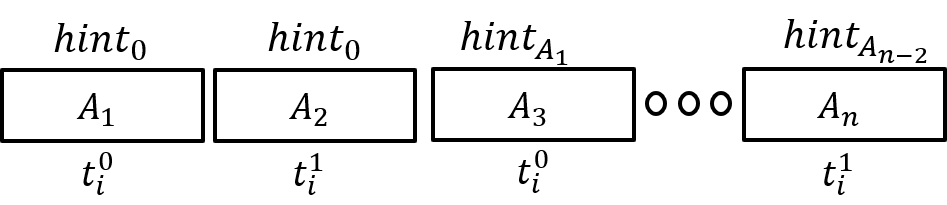
\includegraphics[width=4.2in]{graphics/fast-concurrent/optimisedSimulation.png}
    \caption{Simulation of processing $A=A_1||A_2||\dots||A_n$.}
    \label{fc-fig:optimisedSimulation}
\end{figure}

The simulation uses auxiliary variables oldHint$_i^0$, and oldHint$_i^1$, both initialized to 1.
These variables are updated with the flipping of $cur_i$ (line~\ref{fc-opt:l:swap-local-aux}), such that:
\begin{itemize}
    \item oldHint$_i^0$ is updated to be the current (pre-flip) value of $hint_i$
    \item oldHint$_i^1$ is updated to be the current (pre-flip) value of $oldHint_i^0$
\end{itemize}

%The simulation uses an auxiliary variable $oldHint_i^0$ initialised to 1. This variable is updated
%with the flipping of $cur_i$ (line~\ref{fc-opt:l:swap-local-aux}) with the current value of $hint_i$.

In addition, the simulation uses an auxiliary variable \emph{auxCount$_i$} initialized to 0. This variable is set to
$b$ before the first execution of line~\ref{fc-opt:l:swap-local-aux}, and is never changed after that. 

Finally, the simulation uses two auxiliary variables $PC_i^0$ and $PC_i^1$ to be
program counters for threads $t_i^0$ and $t_i^1$. They are initialized to \emph{Idle}.

We define a mapping $g$ from the state of $OptParSketch$ to the state of $ParSketch$ as follows:
\begin{itemize}
    \item \emph{globalS} in $OptParSketch$ is mapped to \emph{globalS} in $ParSketch$.
    \item localS$_i[j]$ is mapped to $t^j$.localS for $j=0,1$.
    \item counter$_i$ is mapped to $t^{cur_i}$.counter.
    \item auxCount is mapped to $t^{1-cur_i}$.counter.
    \item hint$_i$ is mapped to $t^{cur_i}$.hint and $t^{cur_i}$.prop if $t_i$ is not right before executing line 227,
    otherwise oldHint$_i^0$ is mapped to $t^{cur_i}$.hint and prop$_i$ is mapped to $t^{cur_i}$.prop.
    \item prop$_i$ is mapped to $t^{1-cur_i}$.prop if $t_i$ is not right before executing lines 227-229,
    otherwise oldHint$_i^1$ is mapped to $t^{1-cur_i}$.prop.
    \item oldHint$_i^1$ is mapped to $t^{1-cur_i}$.hint.
\end{itemize}

For example, Figure~\ref{fc-fig:optConcurrentMap} shows a mapping when $cur_i$ equals 0, before executing
line 227. Table~\ref{fc-table:opt-simulation} shows the steps taken by $t_i^0$ and $t_i^1$ when
$cur_i=0$ before line~223.

\begin{figure}[ht]
    \centering
    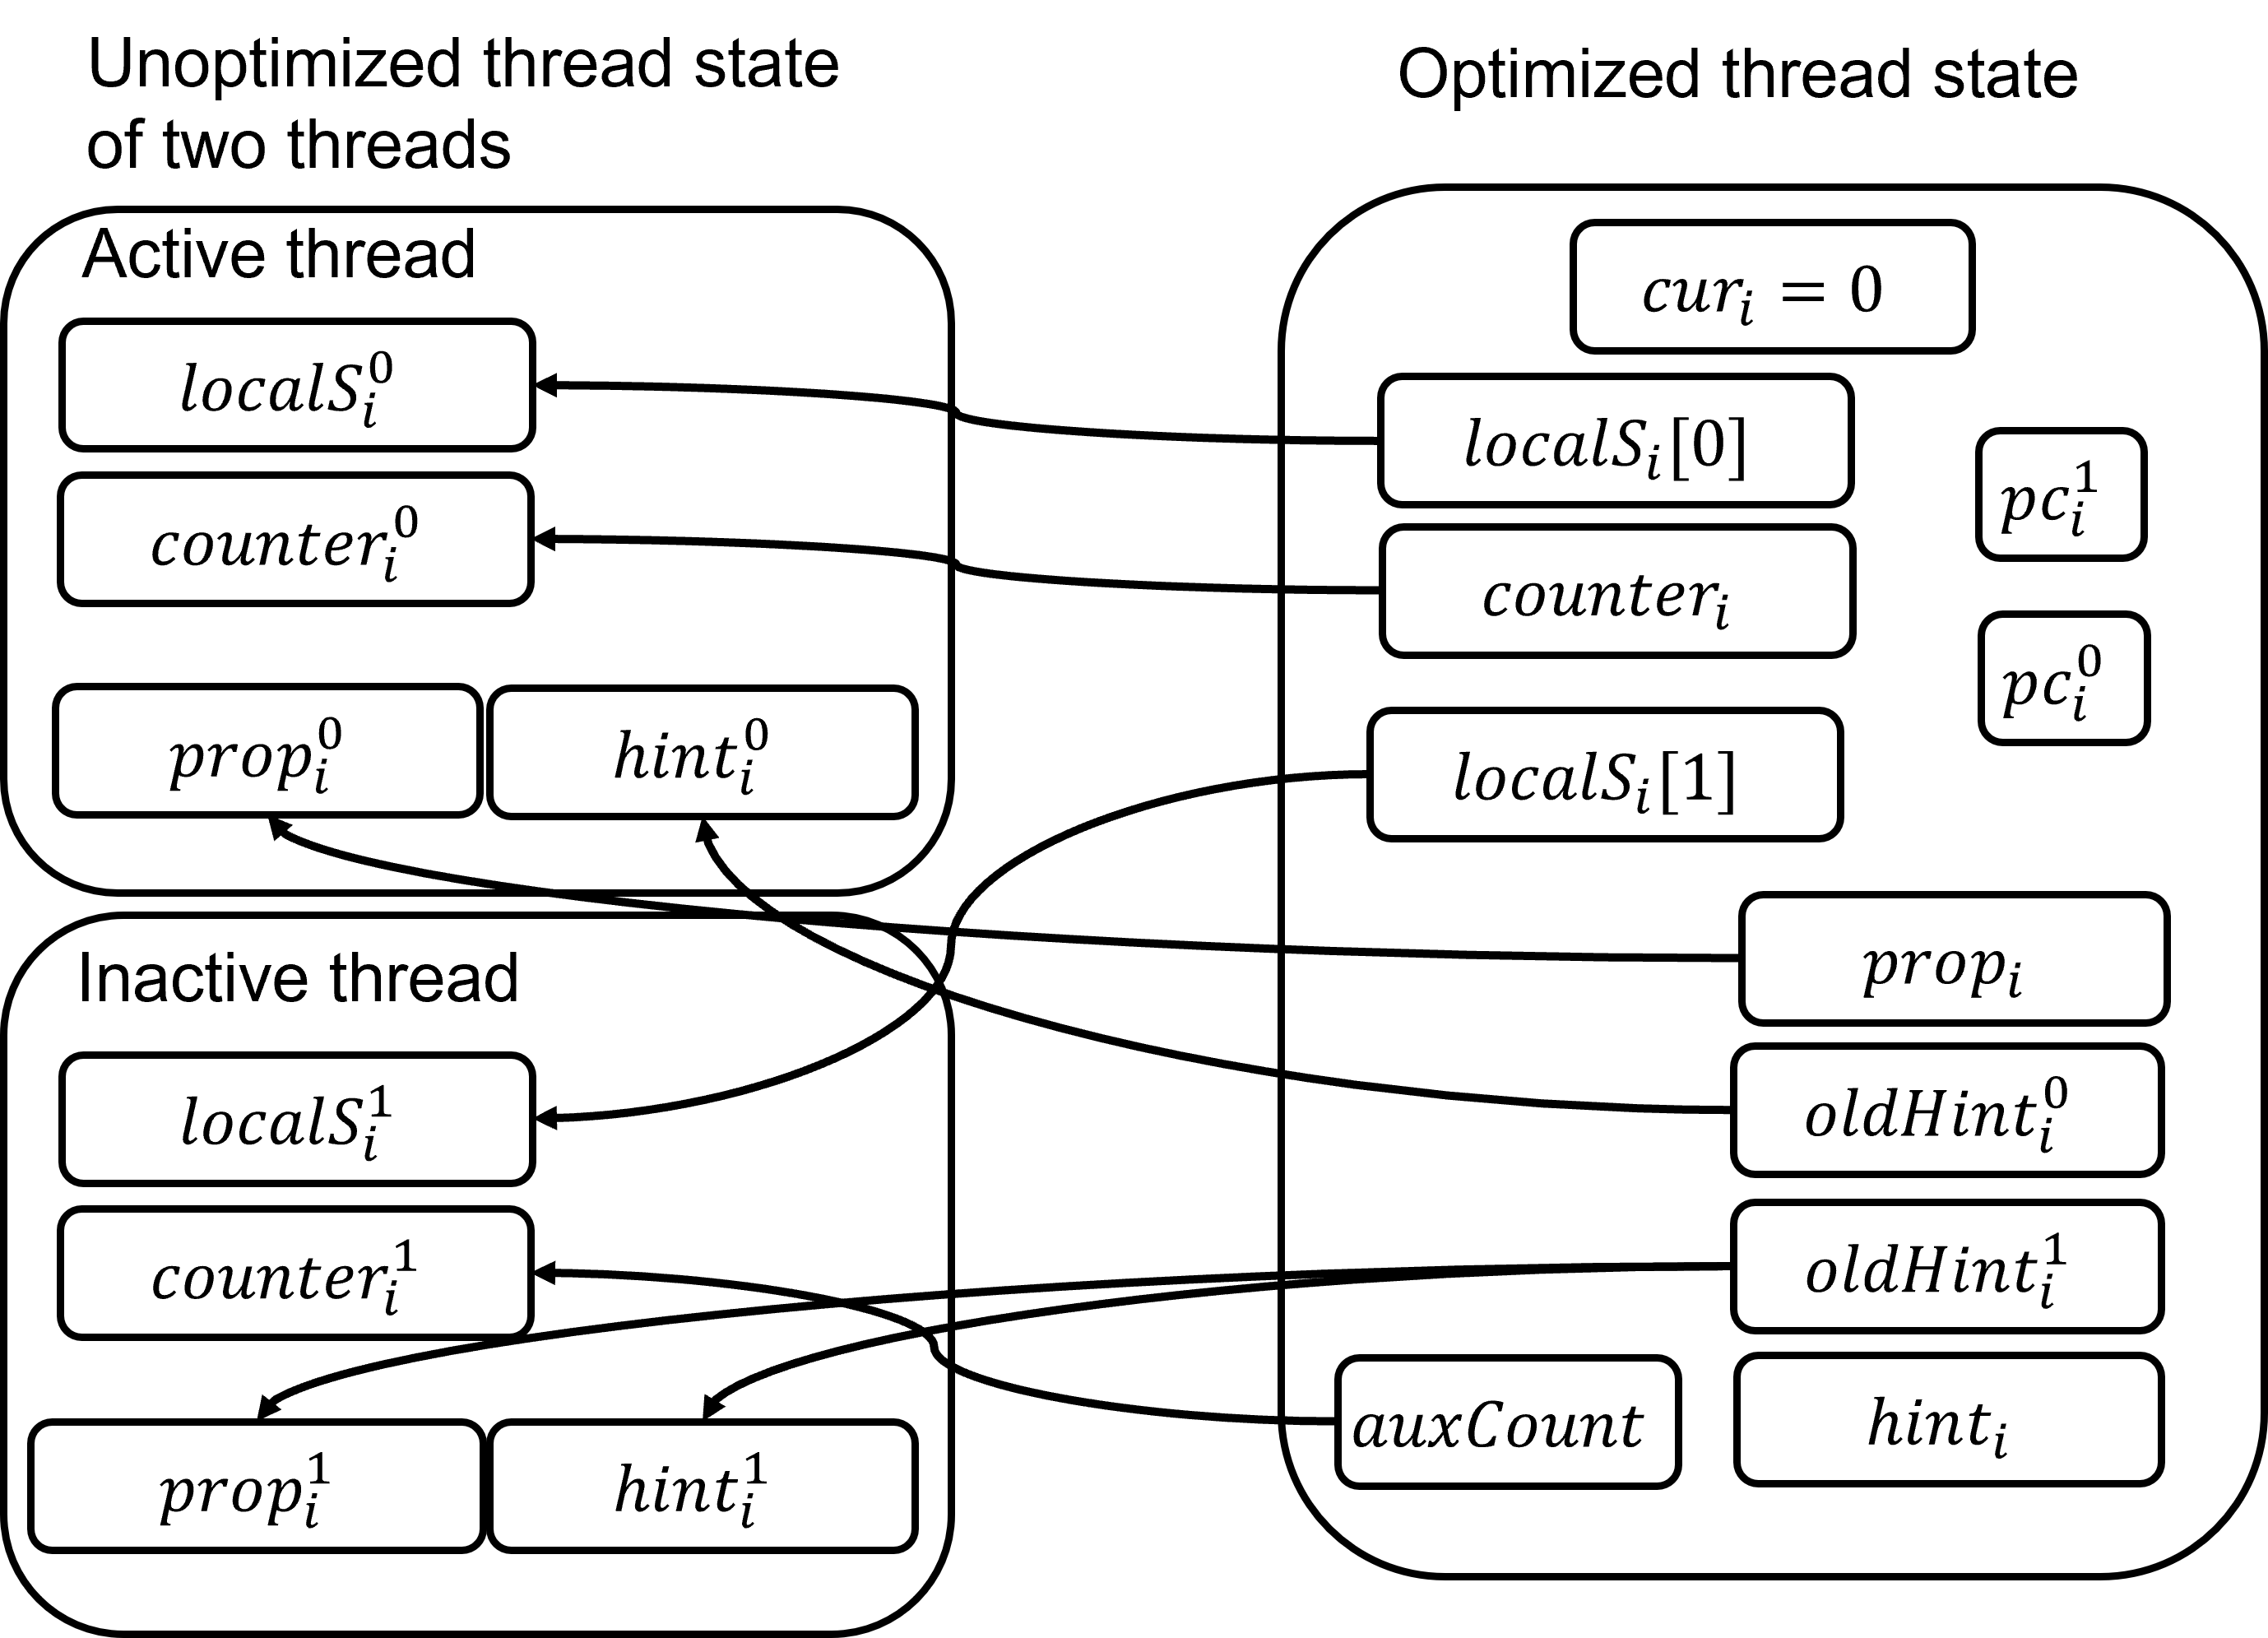
\includegraphics[width=5in]{graphics/fast-concurrent/optConcurrentMap.png}
    \caption{Reference mapping of $g$ when $cur_i$ equals 0 before executing line 227.}
    \label{fc-fig:optConcurrentMap}
\end{figure}

\begin{table}[H]
    \begin{tabular}{c|c|c}
        \emph{OptParSketch} line & \emph{ParSketch} line & Executing thread\\[5pt]
        \hline
        \ref{fc-opt:l:checkfull} & \ref{fc-l:checkfull} & $t_i^0$\\[5pt]
        \ref{fc-opt:l:wait} & \ref{fc-l:wait}& $t_i^1$\\[5pt]
        \ref{fc-opt:l:swap-local-aux} & - & - \\[5pt]
        \ref{fc-opt:l:updateHint} & \ref{fc-l:updateHint} & $t_i^1$\\[5pt]
        \ref{fc-opt:l:zeroCounter} & \ref{fc-l:zeroCounter} & $t_i^1$\\[5pt]
        \ref{fc-opt:l:signal} & \ref{fc-l:signal} & $t_i^0$ 
    \end{tabular}
    \caption{Example for steps taken by $t_i^0$ and $t_i^1$ for each step taken by $t_i$ when $cur_i=0$ before line~\ref{fc-opt:l:checkfull},
    meaning the ``round'' of $b$ updates was ingested by $t_i^0$. On line~\ref{fc-opt:l:swap-local-aux} neither thread takes a step.}
    \label{fc-table:opt-simulation}
\end{table}

We also define the steps taken in $ParSketch$ when $OptParSketch$ takes a step. If a \emph{query} is invoked,
then both algorithms take the same step. If an \emph{update} in invoked, the  \emph{update} is invoked in
$t_i^{cur_i}$ in $ParSketch$. If the counter gets up to $b$ (meaning we get to line~\ref{fc-opt:l:wait}), then
$t_i^{1-cur_i}$ executes line~\ref{fc-l:wait}. When $OptParSketch$ flips $cur_i$ (line~\ref{fc-opt:l:swap-local-aux}),
then neither of the threads $t_i^0$ or $t_i^1$ take a step. Afterwards, lines \ref{fc-opt:l:updateHint} and \ref{fc-opt:l:zeroCounter} execute the corresponding lines (\ref{fc-l:updateHint} and \ref{fc-l:zeroCounter}) 
on thread $t_i^{cur_i}$, and line \ref{fc-opt:l:signal} executes \ref{fc-l:signal} on thread $t_i^{1-cur_i}$.

\begin{lemma}
    $g$ is a simulation relation from $OptParSketch$ to $ParSketch$.
\end{lemma}
\begin{proof}
The proof is by induction on the steps in an execution, for some thread $i$. In the initial state, the mapping trivially holds.
In a given step, we refer to $t_i^{cur_i}$ as the \emph{active} thread and $t_i^{1-cur_i}$ as the \emph{inactive thread}. 
Query threads trivially map to themselves and do not alter the state. We next consider update and propagator threads. 
First, consider the steps of OptParSketch that execute the corresponding step on the active thread.
These are lines 219--223 and 227--228, which directly correspond to lines 119-123 and 127-128 of ParSketch in the
active thread ($t_i^{cur_i}$), and, except in lines 127 and 129, the effected state variables are mapped to the
same state variables in the active thread. So these steps trivially preserve $g$.
Line 124 in \emph{ParSketch} is executed on the inactive thread when \emph{OptParSketch} executes line 229. As after
this step the inactive thread's prop and prop$_i$ are both $0$, so $g$ is preserved. 
Line 125 is executed on the inactive thread, waiting on the same variable, and modifies no variables, so $g$ is preserved.

Line 226 flips $cur_i$ and neither thread takes a step in \emph{ParSketch}. Here, the mappings of $prop$, $hint$, and $counter$ change. 
On this step oldHint$_i^0$ and oldHint$_i^1$ are updated as defined, and as $t_i$ is right before
executing line 227, oldHint$_i^1$ is equal to the inactive thread's ($t_i^{1-cur_i}$) hint, and, as before the step the (now)
inactive thread's prop was equal to hint$_i$, then after this step it is equal to oldHint$_i^0$.
As before the step the (now) active thread's hint was equal to oldHint$_i^0$, after this step it is equal to oldHint$_i^1$. Finally,
as before the step the (now) active thread's prop was equal to prop$_i$, after this step it remains equal to prop$_i$, so this
step preserve $g$.

In line 227, hint$_i$ gets the value of prop$_i$, and the same happens on the active thread. As before this line the
active thread's prop was equal to prop$_i$, after this step the inactive thread's prop and hint are equal to hint$_i$,
preserving $g$.
As the active thread's counter is equal to $counter_i$, line 228 preserves $g$.
The now inactive thread has filled its local sketch, therefore its counter is $b$, which equals
auxCount.  
Finally, the propagator thread’s steps (lines 210-215) execute on the inactive
thread and it is easy to see that all variables accessed in these steps are mapped to the same variables in the inactive thread. 
\end{proof}

Note that the simulation relation uses no prophecy variables, i.e., does not ``look into the future''.
This establishes strong linearizability~\cite{attiya2019putting}, intuitively, because 
the mapping of all ParSketch’s steps -- including linearization points --  to steps in OptParSketch is prefix-preserving.
Since we use two update threads of ParSketch to simulate one thread in OptParSketch, we have proven the following theorem:

\optgenereicstrong*

\section{Deriving error bounds}
\label{fc-sec:error-bounds}

We now show how to translate the $r$-relaxation to a bound on the error of typical sketches.
We consider two types of error anlayzes of existing sketches. In Section~\ref{fc-ssec:theta-analysis}, we consider the 
relative standard error of the $\Theta$ sketch, which was used in the original analysis of the sketch.  
In Section~\ref{fc-ssec:quantiles-error-analysis} we consider PAC sketches, and show generic error bounds for all $r$-relaxed 
implementations of PAC sketches estimating the number of unique elements and quantiles.  

%We bound the error induced by the relaxation on two representative sketches.
%Section~\ref{fc-ssec:RSE-RMSE} formally defines the RSE and RSME metrics.
%Section~\ref{fc-ssec:theta-analysis} discusses the error introduced to the
%expected estimation and RSE of the KMV $\Theta$ sketch.
%Section~\ref{fc-ssec:quantiles-error-analysis} analyses the PAC Quantiles sketch.



\subsection{\texorpdfstring{$\Theta$}{Theta} error bounds}
\label{fc-ssec:theta-analysis}

We bound the error introduced by an $r$-relaxation of the $\Theta$ sketch over a stream with $n$ unique elements and a parameter (sketch size) of $k$. Given
Theorem~\ref{fc-lemma:opt-genereic-strong}, the optimized concurrent sketch's error is bounded
by the relaxation's error bound for $r=2Nb$. We consider strong and weak adversaries,
${\mathcal{A}}_s$ and ${\mathcal{A}}_w$, resp. For the strong adversary we are able to show only numerical
results, whereas for the weak one we show closed-form bounds. The results are summarized in Table~\ref{fc-table:Theta-Error-Summary}.
Our analysis relies on known results from order statistics~\cite{david2004order}.
It focuses on long streams, and assumes $n>k+r$.

%\begin{table}[H]
%    \begin{tabular}{c|cc|cc|cc}
%                      & \multicolumn{2}{c|}{Sequential sketch} & \multicolumn{2}{c|}{Strong adversary ${\mathcal{A}}_s$} & \multicolumn{2}{c}{Weak adversary ${\mathcal{A}}_w$}   \\[5pt]
%                      & Closed-form& Numerical& \multicolumn{2}{c|}{Numerical} & \multicolumn{2}{c}{Closed-form}   \\[5pt]
%                      \hline
%    Expectation & $n$        & $2^{15}$        & \multicolumn{2}{c|}{$2^{15} \cdot 0.995$}          & \multicolumn{2}{c}{$n\frac{k-1}{k+r-1}$} \\[5pt]
%    RSE & $\leq \frac{1}{\sqrt{k-2}}$        & $\leq 3.1\%$        & \multicolumn{2}{c|}{$\leq 3.8\%$}           & \multicolumn{2}{c}{$\leq 2\frac{1}{\sqrt{k-2}}$}         
%    \end{tabular}
%    \caption{Analysis of $\Theta$ sketch with numerical values for $r=8, k=2^{10}, n=2^{15}$.}
%    \label{fc-table:Theta-Error-Summary}
%\end{table}

\begin{table*}[!ht]
    % Table content (and caption)
    \begin{tabular}{c|cc|cc|cc}
        & \multicolumn{2}{c|}{Sequential sketch} & \multicolumn{2}{c|}{Strong adversary ${\mathcal{A}}_s$} & \multicolumn{2}{c}{Weak adversary ${\mathcal{A}}_w$}   \\%[5pt]
        & Closed-form& Numerical& \multicolumn{2}{c|}{Numerical} & \multicolumn{2}{c}{Closed-form}   \\%[5pt]
        \hline
        Expectation & $n$        & $2^{15}$        & \multicolumn{2}{c|}{$2^{15} \cdot 0.995$}          & \multicolumn{2}{c}{$n\frac{k-1}{k+r-1}$} \\%[5pt]
        RSE & $\leq \frac{1}{\sqrt{k-2}}$        & $\leq 3.1\%$        & \multicolumn{2}{c|}{$\leq 3.8\%$}           & \multicolumn{2}{c}{$\leq 2\frac{1}{\sqrt{k-2}}$}         
    \end{tabular}
    \caption{Expectation and RSE of $\Theta$ sketch with numerical values for $r=8, k=2^{10}, n=2^{15}$.}
    \label{fc-table:Theta-Error-Summary}
\end{table*}

We would like to analyze the distribution of the $k^{th}$ largest element in the 
stream that the relaxed sketch processes, as this determines the result returned by the algorithm. 
We cannot use order statistics to analyze this 
because the adversary alters the stream and so the stream seen by the algorithm is not random.
%the $k^{th}$ largest element in the stream is not a random variable. 
However, the stream of hashed unique elements seen by the adversary \emph{is} random. 
Furthermore, if the adversary hides from the algorithm $j$ elements 
smaller than $\Theta$, then the $k^{th}$ largest element in the stream seen
by the  sketch is the $(k+j)^{th}$ largest element in the original stream seen by the adversary. 
This element is a random variable and therefore we can apply order statistics to it.  

We thus model the hashed unique elements in the stream $A$ processed before a given
query as a set of $n$ labelled iid random variables $A_1,\dots,A_n$, taken uniformly 
from the interval $[0,1]$. Note that
$A$ is the stream observed by the reference sequential sketch, and 
also by adversary that hides up to $r$ elements from the relaxed sketch. 
Let $M_{(i)}$ be the $i^{th}$ minimum value among the $n$ random variables $A_1,\dots,A_n$.

Let $est(x) \triangleq \frac{k-1}{x}$ be the estimate computation
with a given $x=\Theta$ (line~\ref{fc-l:update-est} of Algorithm~\ref{fc-alg:composable-theta}).
The sequential (non-relaxed) sketch returns $e=est(M_{(k)})$.
It has been shown that the sketch is unbiased~\cite{KMV}, i.e., $E[e]=n$ the number of unique elements.
Moreover, previous work~\cite{lee-theta} has analyzed the \emph{relative standard error (RSE)} of the sketch, which is 
the standard error divided by the mean, and has shown it to be  
$\textit{RSE}[e]\leq \frac{1}{\sqrt{k-2}}$.
%the supplementary material Section~\ref{fc-ssec:RSE-RMSE}.
%Because this sketch is unbiased, $\textit{RSE}[e]=$\emph{RSME}$[e]$.

In a relaxed history, the adversary chooses up to $r$ variables to hide from the given query so as to maximize its
error. It can also re-order elements, but the state of a $\Theta$ sketch after a set of updates
is independent of their processing order. Let $M^r_{(i)}$ be the $i^{th}$ minimum value among
the hashes seen by the query, i.e., arising in updates that precede the query in the relaxed history.
The value of $\Theta$ is $M^r_{(k)}$, which is equal to $M_{(k+j)}$ for some $0 \leq j \leq r$.
We do not know if the adversary can actually control $j$,
but we know that it can impact it, %and so to bound the error, we can take the worst possible $j$.
%While an arbitrary set of $r$ updates is hidden, in the $\Theta$ sketch,
%only hidden elements that impact $j$ (have hashes smaller than $M^r_{(k)}$)
%affect the query.
and so for our error analysis, we consider strictly stronger adversaries --
we allow both the weak and the strong adversaries to choose the number of hidden
elements $j$. Our error analysis gives an upper bound on the error induced by our adversaries.
Note that the strong adversary can choose $j$ based on the coin flips,
while the weak adversary cannot, and so it cannot distinguish the algorithm state (set of retained elements) from a random one. Since the state is random in all runs, it chooses the same $j$ in all runs.
%The strong adversary knows the hash function and can select $j$ adaptively; the
%weak adversary does not and therefore chooses the same $j$ in all runs.  
%Note that $j$ counts only hidden elements smaller
%than $\Theta$; others are inconsequential.
We show that the largest error is always obtained either for $j=0$ or for $j=r$.
\begin{claim}
    Consider $j$ values $X_i$, $1 \leq i \leq j$, in the interval $[0,1]$,
    let $M_{(i)}$ be the $i^{th}$ minimum value
    among the $j$. The $X_i$ that maximizes $\abs{\frac{k-1}{x}-n}$ for a given $n$
    is either $M_{(0)}$ or $M_{(j)}$.
    \label{fc-claim:max-val}    
\end{claim}
\begin{proof}
    Assume for the sake of contradiction that the variable that
    maximizes $\abs{\frac{k-1}{x}-n}$ is $M_{(i)}$ for $0<i<j$.  We consider two cases:
    \begin{itemize}
    \item If $\frac{k-1}{M_{(i)}} \leq n$, as $M_{(j)} > M_{(i)}$ then $\frac{k-1}{M_{(j)}} < \frac{k-1}{M_{(i)}} \leq n$,
    therefore $\abs{\frac{k-1}{M_{(j)}}-n} > \abs{\frac{k-1}{M_{(i)}}-n}$, which is a contradiction.
    \item If $\frac{k-1}{M_{(i)}} > n$, as $M_{(0)} < M_{(i)}$ then $\frac{k-1}{M_{(0)}} > \frac{k-1}{M_{(i)}} > n$,
    therefore $\abs{\frac{k-1}{M_{(0)}}-n} > \abs{\frac{k-1}{M_{(i)}}-n}$, which is a contradiction.
    \end{itemize}
\end{proof}


\begin{figure}[b]
%\begin{wrapfigure}{r}{0.4\textwidth}
    \begin{center}
        %\vspace{-0.4in}
        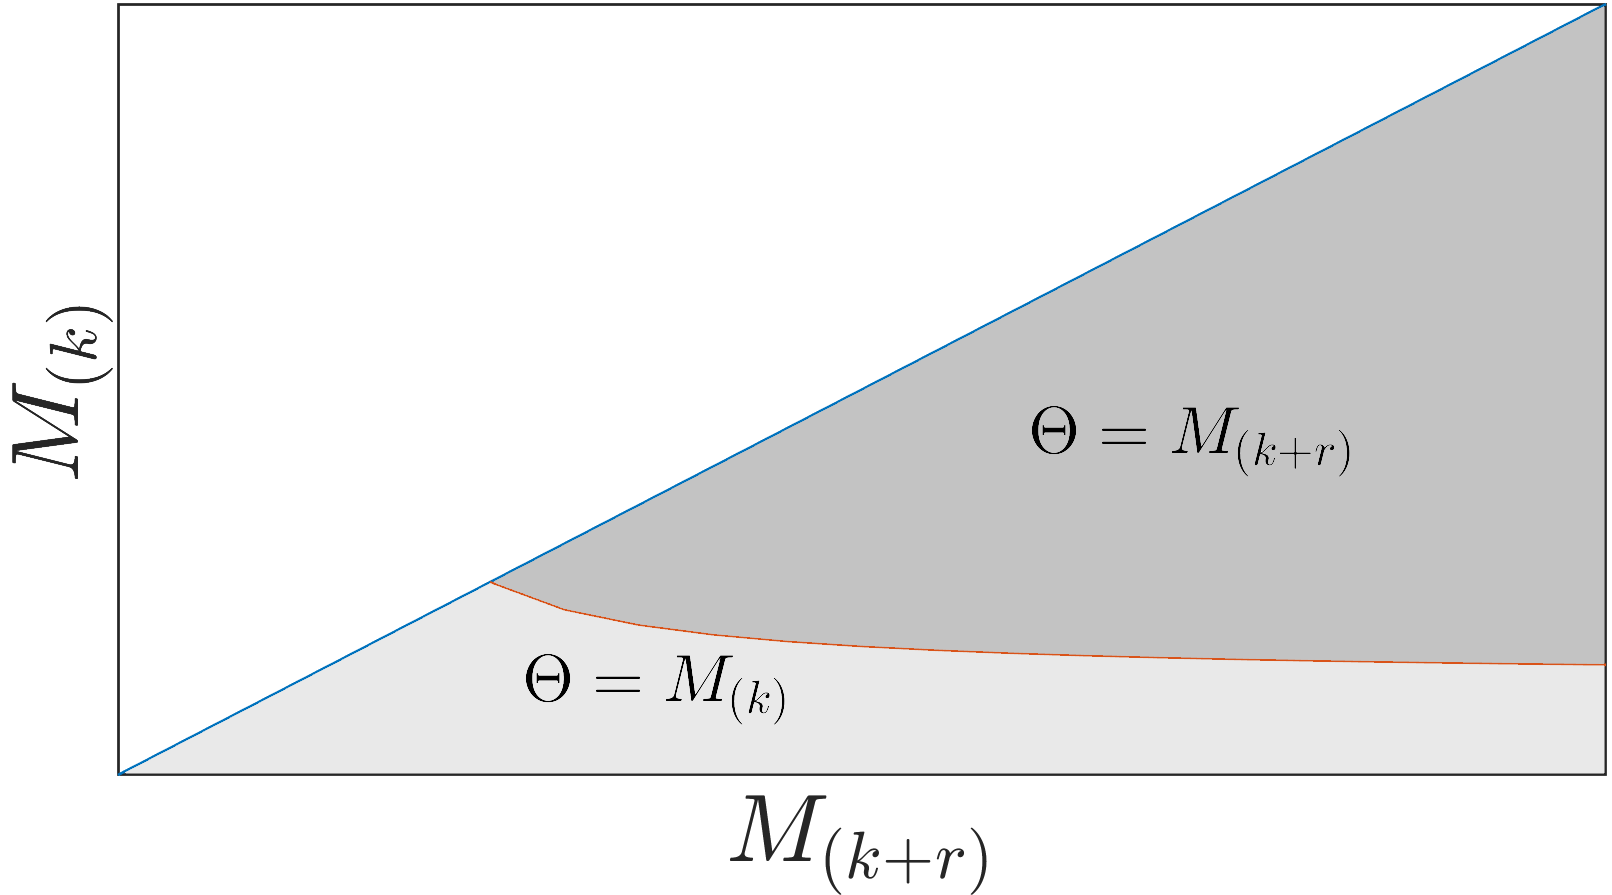
\includegraphics[width=0.38\textwidth]{graphics/fast-concurrent/areaGraph.png}
        %\vspace{-0.2in}
    \end{center}
    \caption{Areas of $M_{(k)}$ and $M_{(k+r)}$. In the dark gray 
    ${\mathcal{A}}_s$ induces $\Theta=M_{(k+r)}$, and in the light gray, $\Theta=M_{(k)}$. The white
    area is not feasible.} %\vspace{-0.1in}
    \label{fc-fig:areaGraph}
%\end{wrapfigure}
\end{figure}

Consider an adversary $\mathcal{A}$ whose estimate is a random variable $e_{\mathcal{A}}$,
characterized by the probability density function $f_{e_{\mathcal{A}}}$.
The expectation of $e_{\mathcal{A}}$ is not necessarily $n$, and so the relative standard error needs to be computed as the error from the desired estimate, $n$, rather than from the expectation. This can be done using the following formula:
\[
    (\textit{RSE}[e_{\mathcal{A}}])^2 = \frac{1}{n^2} \Int_{-\infty}^{\infty} (e - n)^2 \cdot f_{e_{\mathcal{A}}}(e) \,de 
\]
We prove
the following bound:
%Lemma~\ref{fc-lemma:theta-adversary-bound} in the supplementary material Section~\ref{fc-ssec:theta-error-bounds} proves the following bound:
\begin{align*}
    \textit{RSE}[e_{\mathcal{A}}] \leq \sqrt{\frac{\sigma^2(e_{\mathcal{A}})}{n^2}} + \sqrt{\frac{(E[e_{\mathcal{A}}] - n)^2}{n^2}}.
\end{align*}

\begin{lemma}
    The RSE of $e_{\mathcal{A}}$ satisfies the inequality 
    $\textit{RSE}[e_{\mathcal{A}}] \leq \sqrt{\frac{\sigma^2(e_{\mathcal{A}})}{n^2}} + \sqrt{\frac{(E[e_{\mathcal{A}}] - n)^2}{n^2}}$.
    \label{fc-lemma:theta-adversary-bound}
\end{lemma}
\begin{proof}
    \begin{align*}
    \begin{split}
    (\textit{RSE}[e_{\mathcal{A}}])^2 &= \frac{1}{n^2} \Int_{-\infty}^{\infty} (e - n)^2 \cdot f_{e_{\mathcal{A}}}(e) \,de \\
    &= \frac{1}{n^2} \Int_{-\infty}^{\infty} (e - E[e_{\mathcal{A}}] + E[e_{\mathcal{A}}] - n)^2 \cdot f_{e_{\mathcal{A}}}(e) \,de \\
    &\leq \frac{1}{n^2} \Int_{-\infty}^{\infty} \left((e - E[e_{\mathcal{A}}])^2 + (E[e_{\mathcal{A}}] - n)^2 \right)\cdot f_{e_{\mathcal{A}}}(e) \,de \\
    &= \frac{\sigma^2(e_{\mathcal{A}}) + (E[e_{\mathcal{A}}] - n)^2}{n^2} \\
    \text{RSE}[e_{\mathcal{A}}] &\leq \sqrt{\frac{\sigma^2(e_{\mathcal{A}})}{n^2}} + \sqrt{\frac{(E[e_{\mathcal{A}}] - n)^2}{n^2}}
    \end{split}
    \end{align*}
\end{proof}

\paragraph{Strong adversary ${\mathcal{A}}_s$} The strong adversary knows the coin flips in advance, and thus chooses
$j$ to be $g(0, r)$, where $g$ is the
choice that maximizes the error:
\begin{align*}
    g(j_1, j_2) \triangleq \argmax_{j \in \left\{j_1, j_2\right\}} \abs{\frac{k-1}{M_{(k+j)}} - n}.
\end{align*} 

\begin{figure}[b]
%\begin{wrapfigure}{l}{0.4\textwidth}
    \begin{center}
        %\vspace{-0.2in}
        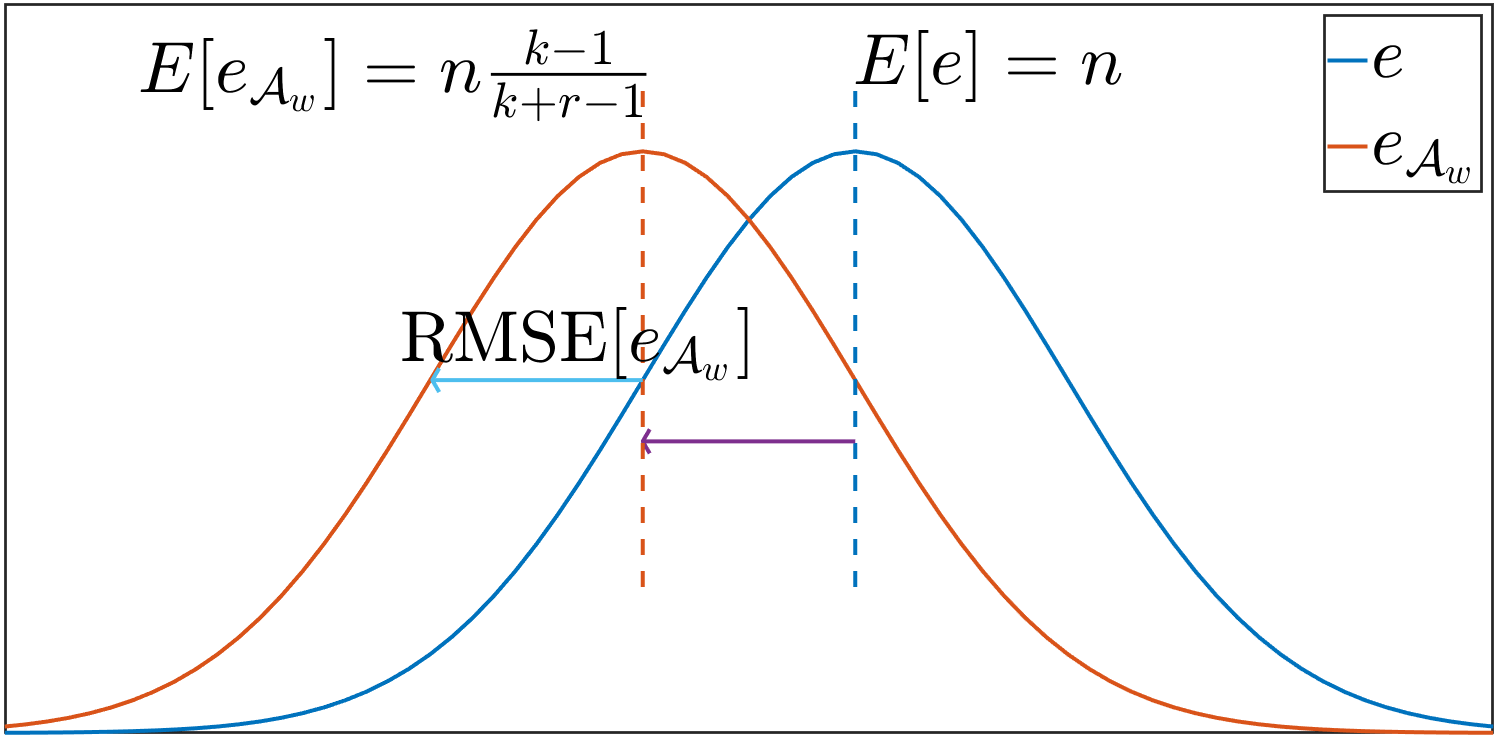
\includegraphics[width=0.39\textwidth]{graphics/fast-concurrent/thetaGraph.png}
        %\vspace{-0.2in}
    \end{center}
    \caption{Distribution of estimators $e$ and $e_{{\mathcal{A}}_w}$. The RSE of $e_{{\mathcal{A}}_w}$ with regards to $n$ is bounded
    by the relative bias plus the RMSE of $e_{{\mathcal{A}}_w}$.}%\vspace{-0.2in}}
    \label{fc-fig:thetaGraph}
%\end{wrapfigure}
\end{figure}

Recall the the ${\mathcal{A}}_s$ knows the oracles coin
flips, therefore knows $M_{(k)}$ and $M_{(k+r)}$, and chooses $M^r_{(k)}$ accordingly. Therefore, our analysis
is on the order statistics of the full stream, as it is this that the adversary sees. From order statistics, the joint probability density
function of $M_{(k)}, M_{(k+r)}$ is:
\begin{align*}
f_{M_{(k)},M_{(k+r)}}(m_k,m_{k+r}) = n!\frac{m_k^{k-1}}{(k-1)!} \frac{(m_{k+r}-m_k)^{r-1}}{(r-1)!}\frac{(1-m_{k+r})^{n-(k+r)}}{(n-(k+r))!}.
\end{align*}

The expectation of $e_{{\mathcal{A}}_s}$ and $e_{{\mathcal{A}}_s}^2$ can be computed as follows:
\begin{equation}
    \begin{split}
    E[e_{{\mathcal{A}}_s}] = \Int_{0}^{1} \Int_{0}^{m_{k+r}} e_{{\mathcal{A}}_s} \cdot f_{M_{(k)},M_{(k+r)}}(m_k,m_{k+r}) \,dm_{k}\,dm_{k+r} \\
    E[e_{{\mathcal{A}}_s}^2] = \Int_{0}^{1} \Int_{0}^{m_{k+r}} \left[e_{{\mathcal{A}}_s} \right] ^2 \cdot f_{M_{(k)},M_{(k+r)}}(m_k,m_{k+r}) \,dm_{k}\,dm_{k+r}
    \end{split}
    \label{fc-eq:strong-expectation}
\end{equation}
Finally, the RSE of $e_{{\mathcal{A}}_s}$ is derived from the standard error of $e_{{\mathcal{A}}_s}$:
\begin{equation}
    \begin{split}
    \text{RSE}[e_{{\mathcal{A}}_s}]^2 &= \frac{1}{n^2}\Int_{0}^{1} \Int_{0}^{m_{k+r}} \left( e_{{\mathcal{A}}_s} - n \right)^2 \cdot f_{M_{(k)},M_{(k+r)}}(m_k,m_{k+r}) \,dm_{k}\,dm_{k+r} \\
    &= \frac{1}{n^2} \Int_{0}^{1} \Int_{0}^{m_{k+r}} \left( e_{{\mathcal{A}}_s} -E[e_{{\mathcal{A}}_s}] + E[e_{{\mathcal{A}}_s}] - n \right)^2 \cdot f_{M_{(k)},M_{(k+r)}}(m_k,m_{k+r}) \,dm_{k}\,dm_{k+r} \\
    &\leq \frac{1}{n^2} \left(\sigma^2(e_{{\mathcal{A}}_s}) + (e_{{\mathcal{A}}_s} - n)^2 \right)\\
    \text{RSE}[e_{{\mathcal{A}}_s}] &\leq \sqrt{\frac{\sigma^2(e_{{\mathcal{A}}_s}) + (e_{{\mathcal{A}}_s} - n)^2}{n^2}} \\
    &\leq \sqrt{\frac{\sigma^2(e_{{\mathcal{A}}_s})}{n^2}} + \sqrt{\frac{(e_{{\mathcal{A}}_s} - n)^2}{n^2}}
    \end{split}
    \label{fc-eq:strong-se-bound}
\end{equation}

In Figure~\ref{fc-fig:areaGraph} we plot the regions where $g$ equals $0$
and $g$ equals $r$, based on their possible combinations of values. The estimate
induced by ${\mathcal{A}}_s$ is $e_{{\mathcal{A}}_s} \triangleq \frac{k-1}{M_{(k+g(0,r))}}$. The expectation
and standard error of $e_{{\mathcal{A}}_s}$ are calculated by integrating over the gray areas
in Figure~\ref{fc-fig:areaGraph} using their joint probability function from order statistics. %In the full paper~\cite{rinberg2019fast} we give
Equations \ref{fc-eq:strong-expectation} and \ref{fc-eq:strong-se-bound} give
the formulas for the expected estimate and its RSE bound, respectively. We do not have
closed-form bounds for these equations. Example numerical results, computed based on Equation~\ref{fc-eq:strong-se-bound}, are
shown in Table~\ref{fc-table:Theta-Error-Summary}.

\paragraph{Weak adversary ${\mathcal{A}}_w$} Not knowing the coin flips, ${\mathcal{A}}_w$ chooses $j$
that maximizes the expected error for a random hash function:
$E[n-est(M^r_{(k)})]=E[n-est(M_{(k+j)})]=n-n\frac{k-1}{k+j-1}$. Obviously this
is maximized for $j=r$. The orange curve in Figure~\ref{fc-fig:thetaGraph} depicts
the distribution of $e_{{\mathcal{A}}_w}$, and the distribution of $e$ is shown in blue.

Recall that ${\mathcal{A}}_w$ always hides $r$ elements smaller than $\Theta$, thus
forcing $M^r_{(k)}=M_{(k+r)}$. Here too our analysis is on the order statistics for the full stream, as this is what the adversary sees.
The expectation of $e_{{\mathcal{A}}_w}$ and $e_{{\mathcal{A}}_w}^2$ is computed using well known equations from order statistics:
\begin{align*}
    E[e_{{\mathcal{A}}_w}]&=E\left[ \frac{k-1}{M_{(k+r)}} \right]=n\frac{k-1}{k+r-1} \\
    E[e_{{\mathcal{A}}_w}^2]&=(k-1)^2\frac{n(n-1)}{(k+r-2)(k+r-1)} \\
    \sigma^2[e_{{\mathcal{A}}_w}] &= E[e_{{\mathcal{A}}_w}^2] - E[e_{{\mathcal{A}}_w}]^2 \\
    &=(k-1)^2\frac{n(n-1)}{(k+r-2)(k+r-1)} - \left(n\frac{k-1}{k+r-1} \right)^2 \\
    &< \frac{n(k-1)^2}{k+r-1}\left[\frac{n}{(k+r-2)(k+r-1)}\right] \\
    \sigma^2[e_{{\mathcal{A}}_w}] &< \frac{n^2}{k+r-2}
\end{align*}

We derive the following equation:
\begin{equation}
    \sqrt{\frac{\sigma^2[e_{{\mathcal{A}}_w}]}{E[e_{{\mathcal{A}}_w}]}}<\frac{1}{k-2}
    \label{fc-eq:ss-rse}
\end{equation}

Finally, the RSE of $e_{{\mathcal{A}}_w}$ is derived from the standard error of $e_{{\mathcal{A}}_w}$, and as $E[e_{{\mathcal{A}}_w}] < n$,
and using the same ``trick'' as in Equation~\ref{fc-eq:strong-se-bound}:
\begin{align*}
    \text{RSE}[e_{{\mathcal{A}}_w}]^2 &= \frac{1}{n^2}\Int_{0}^{1} \left( e_{{\mathcal{A}}_w} - n \right)^2 \cdot f_{M_{(k+r)}}(m_{k+r}) \,dm_{k+r} \\
    &< \frac{1}{n^2} \left(\sigma^2(e_{{\mathcal{A}}_w}) + (E[e_{{\mathcal{A}}_w}] - n)^2 \right)\\
    \text{RSE}[e_{{\mathcal{A}}_w}] &< \sqrt{\frac{\sigma^2(e_{{\mathcal{A}}_w})}{E[e_{{\mathcal{A}}_w}]^2}} + \sqrt{\frac{(E[e_{{\mathcal{A}}_w}] - n)^2}{n^2}}
\end{align*}

Using Equation~\ref{fc-eq:ss-rse}:
\begin{equation}
    \text{RSE}[e_{{\mathcal{A}}_w}] < \sqrt{\frac{1}{k-2}} + \frac{r}{k-2}
    \label{fc-eq:theta-rse-weak-bound}
\end{equation}

%In the full paper~\cite{rinberg2019fast},
%In Equation~\ref{fc-eq:theta-rse-weak-bound}% in the supplementary material Section~\ref{fc-ssec:theta-error-bounds} 
We have shown that the RSE
is bounded by $\sqrt{\frac{1}{k-2}} + \frac{r}{k-2}$ for ${{\mathcal{A}}}_w$.
Thus, whenever $r$ is at most $\sqrt{k-2}$, the RSE of the relaxed
$\Theta$ sketch is coarsely bounded by
twice that of the sequential one. And in case $k \gg r$, the addition to the $RSE$ is negligible.

\subsection{Error bounds for PAC sketches}

We now provide a generic analysis, considering a PAC sketch as a black box. 
Section~\ref{fc-ssec:quantiles-error-analysis} studies quantiles sketches, and 	
in Section~\ref{fc-ssec:pac-unique}, we study PAC sketches estimating the number of unique elements in a stream, e.g., HyperLogLog. 
In both cases, we show that if the sequential sketch's error bound is $\epsilon$, then 
the error of an $r$-relaxed sketch over a stream of size $n$ is bounded by $\epsilon+\frac{r \epsilon}{n}+\frac{r}{n}$. 
This expression tends to  $\epsilon$ as the stream sizes grows to infinity, but may be substantially larger for small streams. 
A system designer can use this formula to determine the adaptation point so that the error is never above a desired threshold. 


\subsubsection{Quantiles error bounds}
\label{fc-ssec:quantiles-error-analysis}

%\begin{wraptable}{c}{0pt}
%    \begin{tabular}{c|ccc}
%    Quantile        & Sequential                                   & Weak adversary ${\mathcal{A}}_w$ \\[5pt]
%    \hline
%    $\phi \leq 0.5$ & $\phi n \pm \epsilon n$ & $\phi n + (1-\phi)r \pm \epsilon(n - r)$ \\[5pt]
%    $\phi > 0.5$    & $\phi n \pm \epsilon n$ & $\phi n -\phi r \pm \epsilon(n - r)$
%    \end{tabular}
%    \caption{Quantiles sketch: Result range with probability $1-\delta$, for sequential sketch and $r$-relaxation with weak adversary,
%    and $\epsilon_r=\epsilon - \frac{r \epsilon}{n} + \frac{r}{n}$.}
%    \label{fc-table:Quantiles-Error-Summary}
%\end{wraptable}

\iffalse
\begin{wraptable}{c}{0pt}
    \begin{tabular}{c|ccc}
    Quantile        & Sequential                                   & Weak adversary ${\mathcal{A}}_w$ \\[5pt]
    \hline
    $\phi $ & $\phi n \pm \epsilon n$ & $\phi n \pm \left(\epsilon - \frac{r \epsilon}{n} + \frac{r}{n}\right) n$ 
    \end{tabular}
    \caption{Quantiles sketch: Result range with probability $1-\delta$, for sequential sketch and $r$-relaxation with weak adversary,
    and $\epsilon_r=\epsilon - \frac{r \epsilon}{n} + \frac{r}{n}$.}
    \label{fc-table:Quantiles-Error-Summary}
\end{wraptable}
\fi

We now analyze the error for any implementation of the sequential Quantiles sketch, provided that the sketch is
\emph{PAC}, meaning that a query for quantile $\phi$
returns an element whose rank is between $(\phi-\epsilon)n$ and $(\phi+\epsilon)n$ with 
probability at least $1-\delta$ for some parameters $\epsilon$ and $\delta$. We show that the $r$-relaxation of
such a sketch returns an element whose rank is in the range $(\phi \pm\epsilon_r)n$ with probability at
least $1-\delta$ for $\epsilon_r=\epsilon - \frac{r \epsilon}{n} + \frac{r}{n}$.

Although the desired summary is order agnostic here too, Quantiles sketch implementations (e.g., \cite{agarwal2013mergeable})
are sensitive to the processing order. In this case, advance knowledge of the coin flips can increase the error
already in the sequential sketch. Therefore, we do not consider a strong adversary, but rather discuss only the weak one.
Note that the weak adversary attempts to maximize $\epsilon_r$.

Consider an adversary that knows $\phi$ and chooses to hide
$i$ elements below the $\phi$ quantile and $j$ elements above it, such that $0\leq i+j\leq r$. The rank of the element
returned by the query among the $n-(i+j)$ remaining elements is in the range 
$\phi(n-(i+j)) \pm \epsilon(n-(i+j))$.
There are $i$ elements below this quantile that are missed, and therefore its rank in the original stream is in the range:
\begin{equation}
    \left[ (\phi-\epsilon)(n-(i+j)) + i , (\phi+\epsilon)(n-(i+j)) + i \right].
    \label{fc-eq:rank-range}
\end{equation}

This can be rewritten as:
\begin{equation}
\begin{split}
    [\phi n - (\phi j - (1-\phi)i+\epsilon(n-(i+j))), \\
    \phi n + ((1-\phi)i - \phi j +\epsilon(n-(i+j))) ] 
\end{split}
    \label{fc-eq:rank-range-2}
\end{equation}

Note that this interval is symmetric around $\phi(n-(i+j)) + i$.
The adversary attempts to maximize the distance of the edges of this interval from the true rank,
(i.e., maximize $\epsilon_r$). The distance between the central points is:
\begin{align*}
    \abs{\phi n + (1-\phi)i - \phi j - \phi n}=\abs{(1-\phi)i - (\phi)j}.
\end{align*}
Given that $0\leq i+j\leq r$, we show that this expression is maximized
for $i+j=r$.
\begin{claim}
    Given $0\leq i,j$ such that $0\leq i+j\leq r$, the expression $\abs{(1-\phi)i - (\phi)j}$
    is maximized for $(i,j)=(x,y)$ such that $x+y=r$.
    \label{fc-claim:sum-r}
\end{claim}
\begin{proof}
    Assume by contradiction that the expression given in the claim is maximized for $(x,y)$ such that $x+y=r'<r$. Denote
    $r'=r-k$. We consider two cases for the expression $(1-\phi)i - (\phi)j$.

    If $(1-\phi)x - (\phi)y \geq 0$, then $(1-\phi)(x+k) - (\phi)y \geq (1-\phi)x - (\phi)y >0$. In this
    case denote $x'=x+k$ and $y'=y$.

    If $(1-\phi)x - (\phi)y < 0$, then $(1-\phi)x - (\phi)(y+k) \leq (1-\phi)x - (\phi)y < 0$. In this
    case denote $x'=x$ and $y'=y+k$.

    In both cases we found $(x',y')$ such that $x'+y'=r$ and the expression $\abs{(1-\phi)i - (\phi)j}$
    is maximized for $(i,j)=(x',y')$.
\end{proof}

%This is proven in Claim~\ref{fc-claim:sum-r} in the supplementary material Section~\ref{fc-ssec:quantiles-sketch-error-bounds}.
By substituting $j=r-i$ into the error formula, we get:
\begin{align*}
    \abs{(1-\phi)i - (\phi)(r-i)}=\abs{i - \phi r}.
\end{align*}
As $0\leq \phi \leq 1$, the following claim follows immediately:
\begin{claim}
    For $\phi \leq 0.5$ the adversary maximizes the distance by choosing $i=r$ (and therefore $j=0$)
    and for $\phi > 0.5$ the adversary maximizes the error by choosing $i=0$ (and therefore $j=r$).
    \label{fc-clm:quantiles-relaxation-choice}
\end{claim}

We begin by analyzing the range given in Equation~\ref{fc-eq:rank-range-2} for $0 \leq \phi \leq 0.5$.

\begin{claim}
    For $0 \leq \phi \leq 0.5$ and $i,j>0$ such that $0 \leq i+j \leq r$ and $\epsilon < 0.5$, then: (1) $(1-\phi)i-\phi j + \epsilon(n-(i+j)) \leq (1-\phi) r + \epsilon(n-r)$,
    and (2) $\phi j - (1-\phi)i + \epsilon(n-(i+j)) \leq (1-\phi) r + \epsilon(n-r)$.
    \label{fc-clm:quantiles-bottom-half}
\end{claim}
\begin{proof}
    As $\phi \leq 0.5$, and $\epsilon \ll 0.5$ then $1-\phi-\epsilon > 0$. As $0 \leq i+j \leq r$, then $i \leq r$.
    \begin{align}
        f(i,j)&=(1-\phi)i-\phi j + \epsilon(n-(i+j)) \leq (1-\phi)i + \epsilon(n-i) \leq (1-\phi-\epsilon)i +\epsilon n \\
        &\leq (1-\phi-\epsilon)r +\epsilon n = (1-\phi)r+\epsilon(n-r) = f(r,0)
    \end{align}

    As $\phi \leq 0.5$, then $\phi \leq 1-\phi$, and as As $0 \leq i+j \leq r$, then $i \leq r$
    \begin{align}
        \phi j - (1-\phi)i + \epsilon(n-(i+j)) \leq (1-\phi )j +\epsilon (n-j)  \leq (1-\phi) r + \epsilon (n-r)
    \end{align}
\end{proof}


We next analyze the same range for $0.5 < \phi \leq 1$.

\begin{claim}
    For $0.5 < \phi \leq 1$ and $i,j>0$ such that $0 \leq i+j \leq r$ and $\epsilon < 0.5$, then: (1) $\phi i - (1-\phi)j + \epsilon(n-(i+j)) \leq \phi r + \epsilon(n-r)$, 
    and (2) $(1-\phi)i - \phi j + \epsilon(n-(i+j)) \leq \phi r + \epsilon(n-r)$.
    \label{fc-clm:quantiles-top-half}
\end{claim}
\begin{proof}
    As $\phi > 0.5$, and $\epsilon \ll 0.5$ then $\phi-\epsilon > 0$. As $0 \leq i+j \leq r$, then $i \leq r$.
    \begin{align}
        f(i,j)=\phi i - (1-\phi)j + \epsilon(n-(i+j)) \leq \phi i +\epsilon (n-i) \leq (\phi - \epsilon)i + \epsilon n \leq \phi r + \epsilon(n-r) = f(r,0)
    \end{align}

    As $\phi > 0.5$, then $(1-\phi) \leq \phi$, and as As $0 \leq i+j \leq r$, then $i \leq r$
    \begin{align}
        (1-\phi)i - \phi j + \epsilon(n-(i+j)) \leq \phi i + \epsilon (n-i) \leq \phi r + \epsilon(n-r)
    \end{align}
\end{proof}

Putting the two claims together we get:

\begin{claim}
    For $0 \leq \phi \leq 1$ and $i,j>0$ such that $0 \leq i+j \leq r$ and $\epsilon \ll 0.5$, then: (1) $\phi i - (1-\phi)j + \epsilon(n-(i+j)) \leq r + \epsilon(n-r)$,
    and (2) $(1-\phi)i - \phi j + \epsilon(n-(i+j)) \leq r + \epsilon(n-r)$.
    \label{fc-clm:helper}
\end{claim}
\begin{proof}
    From Claim~\ref{fc-clm:quantiles-bottom-half}, for $0 \leq \phi \leq 0.5$ then both inequalities are bounded by $(1-\phi) r + \epsilon(n-r)$, and as $\phi \geq 0$ then
    $(1-\phi) r + \epsilon(n-r) \leq r + \epsilon(n-r)$.

    From Claim~\ref{fc-clm:quantiles-top-half}, for $0.5 < \phi \leq 1$ then both inequalities are bounded by $\phi r + \epsilon(n-r)$, and as $\phi \leq 1$ then
    $\phi r + \epsilon(n-r) \leq r + \epsilon(n-r)$.
\end{proof}

Finally, we prove a bound on the rank of the element returned. 
\begin{lemma}
    Given parameters $(\epsilon,\delta)$ if $\epsilon<0.5$, then the $r$-relaxed
    quantiles sketch returns an element whose rank is
    between $(\phi-\epsilon_r)n$ and $(\phi+\epsilon_r)n$ with probability at
    least $1-\delta$, where $\epsilon_r=\epsilon - \frac{r \epsilon}{n} + \frac{r}{n}$.
    \label{fc-lemma:quantiles-weak-adversary}
\end{lemma}
\begin{proof}
    Given parameters $(\epsilon,\delta)$, and given that the adversary hides $i$ elements below the
    $\phi$ quantile and $j$ elements above it, such that $0\leq i+j\leq r$, the rank of the element returned
    by the query is in the range given in Equation~\ref{fc-eq:rank-range-2} w.p. at least $1-\delta$:
    \begin{align*}
        \left[\phi n - (\phi j - (1-\phi)i+\epsilon(n-(i+j))), \phi n + ((1-\phi)i - \phi j +\epsilon(n-(i+j))) \right].
    \end{align*}

    From Claim~\ref{fc-clm:helper}, this range is contained within the range:
    \begin{align*}
        \left[\phi n - (r + \epsilon(n-r)), \phi n + (r + \epsilon(n-r)) \right].
    \end{align*}
    Which can be rewritten as the range $\left(\phi \pm \left(\epsilon - \frac{r \epsilon}{n} + \frac{r}{n}\right)\right)n$.
    Meaning the rank of the element returned is between $(\phi-\epsilon_r)n$ and $(\phi+\epsilon_r)n$ with probability at
    least $1-\delta$, where $\epsilon_r=\epsilon - \frac{r \epsilon}{n} + \frac{r}{n}$.
\end{proof}

%In the full paper~\cite{rinberg2019fast}, we
%In Lemma~\ref{fc-lemma:quantiles-weak-adversary} in the supplementary material Section~\ref{fc-sec:appendix-error-bounds} we
We have shown that the $r$-relaxed sketch returns an element whose rank is
%show that the $r$-relaxed sketch returns an element whose rank is
between $(\phi-\epsilon_r)n$ and $(\phi+\epsilon_r)n$ with probability at
least $1-\delta$, where $\epsilon_r=\epsilon - \frac{r \epsilon}{n} + \frac{r}{n}$. Thus
the impact of the relaxation diminishes as $n$ grows.
%The ranges are illustrated in Figure~\ref{fc-fig:quantiles-range}.

\subsubsection{Count unique elements error bounds}
\label{fc-ssec:pac-unique}

Finally, we consider the error of any implementation of a count unique elements sketch, provided
that the sketch is PAC. In this case, for a stream with $n$ unique elements, the query returns an estimate $e$ which is in between
$(1-\epsilon)n$ and $(1+\epsilon)n$ with probability at least $1-\delta$ for some parameters
$\epsilon$ and $\delta$. We show that the $r$-relaxation of such a sketch returns an estimate
is in the range $(1 \pm \epsilon_r)n$ with probability at least $1-\delta$
for $\epsilon_r=\epsilon+\frac{r \epsilon}{n}+\frac{r}{n}$.

As in a Quantiles sketch, advance knowledge of the coin flip can increase the
error already in the sequential sketch. Therefore, here too, we focus on a weak adversary.  
As above, the adversary hides either no
elements or $r$ elements. If the adversary hides $r$ elements, the estimate returned is in the range
$(1 \pm \epsilon)(n-r)$.

The adversary thus chooses whether to hide $r$ elements or not based on which estimate maximizes the
error $|n-e|$. In either case, with probability at least $1-\delta$ the estimate is between
$(1-\epsilon)(n-r)$ and $(1+\epsilon)n$. This range is contained in the range
$n\left(1 \pm \left(\epsilon+\frac{r \epsilon}{n}+\frac{r}{n}\right)\right)$. We can define
$\epsilon_r \triangleq \epsilon+\frac{r \epsilon}{n}+\frac{r}{n}$. Note that, as in the case of the
Quantiles sketch, here too, the impact of the relaxation diminishes as $n$ grows.

\section{\texorpdfstring{$\Theta$}{Theta} sketch evaluation}
\label{fc-sec:eval}

This section presents an evaluation of an implementation of our algorithm for the $\Theta$ sketch.
Section~\ref{fc-ssec:setup-and-methodology} presents the methodology for the analysis.
Section~\ref{fc-ssec:results} shows the results under different
workloads and scenarios. Finally, Section~\ref{fc-ssec:tradeoffs} discusses the tradeoff between
accuracy and throughput.

\subsection{Setup and methodology}
\label{fc-ssec:setup-and-methodology}

Our implementation~\cite{ConcurrentThetaImp} extends the code in Apache DataSketches~\cite{DataSketches}, a Java
open-source library of stochastic streaming algorithms. The $\Theta$ sketch there differs slightly
from the KMV $\Theta$ sketch we used as a running example, and is based on a HeapQuickSelectSketch family.
In this version, the sketch stores between $k$ and $2k$ items, whilst keeping $\Theta$ as the $k^{\text{th}}$
largest value. When the sketch is full, it is sorted and the largest $k$ values are discarded.

Concurrent $\Theta$ sketch is generally available in the Apache DataSketches
library since V0.13.0. The sequential implementation and the sketch at the core of the global sketch
in the concurrent implementation are the both \\ HeapQuickSelectSketch, which is the default sketch family.


We implement a limit for eager propagation as a function
of the configurable error parameter $\epsilon$; the function we use is $2 / \epsilon^2$. The local sketches define $b$
as a function of $k$, $\epsilon$, and $N$ (the number of writer threads) such that the error induced by
the relaxation when in the lazy propagation mode does not exceed $e$ using Equation~\ref{fc-eq:theta-rse-weak-bound}.
Thus the total error is bounded by $\max\{\epsilon + \frac{1}{\sqrt{k}}, \frac{2}{\sqrt{k}}\}$.

Eager propagation, as described in the pseudo-code, requires context switches incurring a high overhead. In the
implementation, either the local thread itself executes every update to the global sketch (equivalent to a
buffer size of 1) or lazily delegates updates to a background thread. While the sketch is in eager propagation
mode, the global sketch is protected by a shared boolean flag. When the sketch switches to estimate mode it
is guaranteed that no eager propagation gets through; instead local threads pass the buffer via lazy propagation.
This implementation ensures that: (a) local threads avoid costly context switches when the sketch is small, and (b)
lazy propagation by a background thread is done without synchronization.

Unless stated otherwise, we use k=4096, which is commonly used~\cite{DataSketches} for the $\Theta$ sketch.
The sequential sketch’s RSE with this buffer size is $0.031$ with a probability of at
least $0.95$. In the concurrent sketch, we chose to limit the error to $\epsilon = 0.04$ with the
same probability. Given a particular number of threads $N$, $b$ is derived according to
Equation~\ref{fc-eq:theta-rse-weak-bound} with $r = 2Nb$. Recall that the analysis in Section~\ref{fc-ssec:theta-analysis}
(including this equation) is
conditioned on the assumption that $n > k + r$. Therefore, if we would set the eager
adaptation threshold to $k+2Nb$, we would get the same error bound for any sketch size.
However, this is a conservative choice. We experiment with a threshold of $1250$,
and show that empirically, the error is reasonable with this choice. In general, this is
a configurable parameter, which can be used by system designers to navigate the tradeoff between
accuracy and performance.

%Unless otherwise stated, sketches are configured with $k=4096$, and $\epsilon=0.04$; thus the sketch swithces
%from eager propagation to lazy after $2/\epsilon^2=1250$ unique elements, and
%$b$ is set (by the implementation) to a value between $1$ and $5$ to accommodate the
%error bound.
Our first set of tests run on a 12-core Intel Xeon E5-2620 machine -- this machine is similar
to that which is used by production servers. For the scalability evaluation (shown in the introduction) we use a 32-core Intel Xeon
E5-4650 to get a large number of threads. Both machines have hyper-threading disabled, as it introduces
non-monotonic effects among threads sharing a core.

We focus on two workloads: (1) write-only -- updating a sketch with a stream of unique values; (2) mixed
read-write workload -- updating a sketch with background reads querying the number of unique values in
the stream. Background reads refer to dedicated threads that occasionally (with $1$ms pauses) execute a query.
These workloads simulate scenarios where updates are constantly streaming from
a feed or multiple feeds, while queries arrive at a lower rate.

To run the experiments we employ a multi-thread extension of the characterization
framework. This is the Apache DataSketch evaluation benchmark suite, which measures
both the speed and accuracy of the sketch. 

For measuring write throughput, the sketch is fed with a continuous data stream. The size of
the stream varies from 1 to 8M unique values. For each size $x$ we measure the time $t$ it takes to feed the
sketch $x$ unique values, and present it in term of throughput ($x/t$).
To minimize measurement noise, each point on the graph represents an average of
many trials. Small stream sizes tend to suffer more from measurement noise, so
the number of trials is very high (in the millions). As the stream size gets larger,
the number of trials gradually decreases down to 16 in the largest stream.
%The number of trials is very high
%($2^{18}$) for points at the low end of the graph. It gradually decreases as the size of the
%sketch increases. At the high end (at 8M values per trial) the number of trials is 16. This is because
%smaller stream sizes tend to suffer more from measurement noise.

Note that accuracy is measured relative to the number of unique elements ingested to the
sketch before a query in some linearization; because we cannot empirically deduce the
linearization point of a query that is run in parallel with updates, the metric is only
well-defined when the query is not concurrent to any update. Therefore, we measure
accuracy only in a single-thread environment, where we periodically interleave queries
with updates of the same thread. The accuracy with more threads can be extrapolated
from these measurements based on the theoretical analysis.

As in the performance evaluations, the $x$-axis represents the number of unique values fed into the sketch
by a single writing thread. For each size $x$, one trial logs the estimation result after feeding $x$
unique values to the sketch. In addition, it logs the Relative Error (RE) of the estimate, where
$\mathit{RE} = \mathit{MeasuredValue}/\mathit{TrueValue} - 1$. This trial is repeated 4K times,
logging all estimation and $\mathit{RE}$ results. The curves depict the mean and some
quantiles of the distributions of error measured at each $x$-axis point on the graph, including the median. 
This type of graph is called a ``pitchfork''.


\subsection{Results}
\label{fc-ssec:results}

\paragraph{Accuracy results}
Our first set of tests runs on a 12-core Intel Xeon E5-2620 machine. The accuracy results for the concurrent $\Theta$ sketch
without eager propagation are presented in Figure~\ref{fc-fig:accuracy}. There are two interesting phenomena worth noting.
First, it is interesting to see empirical evaluation reflecting the theoretical analysis presented in Section~\ref{fc-ssec:theta-analysis},
where the pitchfork is distorted towards underestimating the number of unique values. Specifically, the mean relative error is smaller
than $0$ (showing a tendency towards underestimating), and the relative error in all measured quantiles tends to be smaller
than the relative error of the sequential implementation.

Second, when the stream size is less than $2k$, $\Theta=1$ and the estimation is the number of values propagated to the
global sketch. If we forgo eager propagation, the number of values in the global sketch depends on the delay in propagation. The
smaller the sketch, the more significant the impact of the delay, and the mean error reaches as high as $94\%$ (the error in
the figure is capped at $10\%$). As the number of propagated values approaches $2k$, the delay in propagation is less significant, and
the mean error decreases. This excessive error is remedied by the eager propagation mechanism. The maximum error allowed by
the system is passed as a parameter to the concurrent sketch, and the global sketch uses eager propagation to stay within
the allowed error limit. Figure~\ref{fc-fig:accuracy-adaptive} depicts the accuracy results when applying eager
propagation. The figures are similar when the sketch begins lazy propagation, and the error stays within the $0.04$
limit as long as eager propagation is used.

\begin{figure*}[tb]
    \setlength{\abovecaptionskip}{0pt}
    \setlength{\belowcaptionskip}{0pt}
    \setlength\textfloatsep{0pt}
    \centering
    \begin{subfigure}{\columnwidth}\centering
    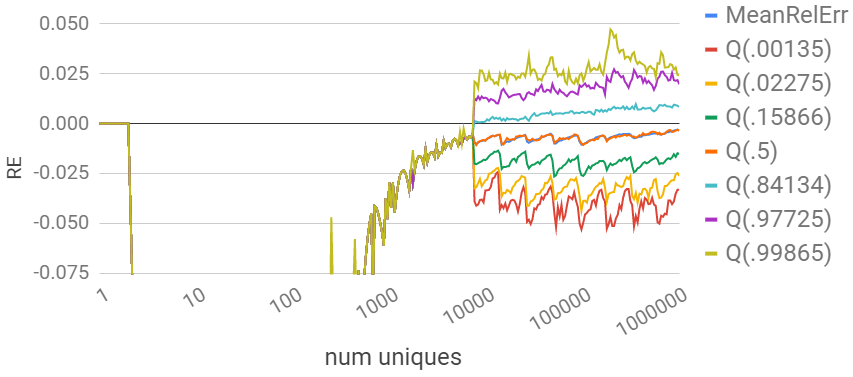
\includegraphics[width=\textwidth]{graphics/fast-concurrent/theta-accuracy.PNG}
    \caption{No eager propagation ($\epsilon=1.0$)}
    \label{fc-fig:accuracy}
    \end{subfigure}
    \begin{subfigure}{\columnwidth}\centering
    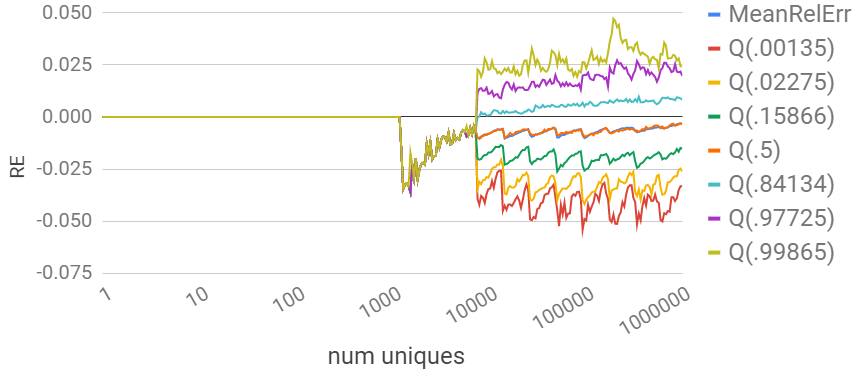
\includegraphics[width=\textwidth]{graphics/fast-concurrent/theta-accuracy-adaptive.PNG}
    \caption{With eager propagation, error bound defined by $\epsilon=0.04$}
    \label{fc-fig:accuracy-adaptive}
    \end{subfigure}
      \caption{Concurrent $\Theta$ measured quantiles vs RE, $k = 4096$.}
      \label{fc-fig:accuracy-res}
\end{figure*}

\paragraph{Write-only workload}
Figure~\ref{fc-fig:throughput:native} presents throughput measurements for a write-only workload. The results are shown in $\log \log$ scale.
Figure~\ref{fc-fig:throughput:large} zooms-in on the throughput of large streams. As explained in Section~\ref{fc-ssec:setup-and-methodology},
we compare the concurrent implementation to a lock-based approach. The number of threads in both implementations refers to the
number of worker threads; there can be arbitrarily many reader threads.

When considering large stream sizes, the concurrent implementation scales with the number of threads, peaking at
almost $300$M operations per second with $12$ threads. The performance of the lock-based implementation, on the other hand,
degrades as the contention on the lock increases.
%Its peak performance is $25$M operations per second with a single thread.
At the peak measured performance the single threaded concurrent $\Theta$ sketch outperforms the single
threaded lock based implementation by $12$x, and with $12$ threads by more than $45$x.
%Namely, with a single thread, the concurrent $\Theta$ sketch outperforms the lock-based implementation
%by $12$x, and with $12$ threads by more than $45$x. 

For small streams, wrapping a single thread with a lock is the most efficient method. Once the stream
contains more than $200$K unique values, using a concurrent sketch with $4$ or more local threads is more efficient.
The crossing point where a single local buffer is faster than the lock-based implementation is around $700$K unique values.
 
\begin{figure*}[tb]
\setlength{\abovecaptionskip}{0pt}
\setlength{\belowcaptionskip}{0pt}
\setlength\textfloatsep{0pt}
\centering
\begin{subfigure}{\columnwidth}\centering
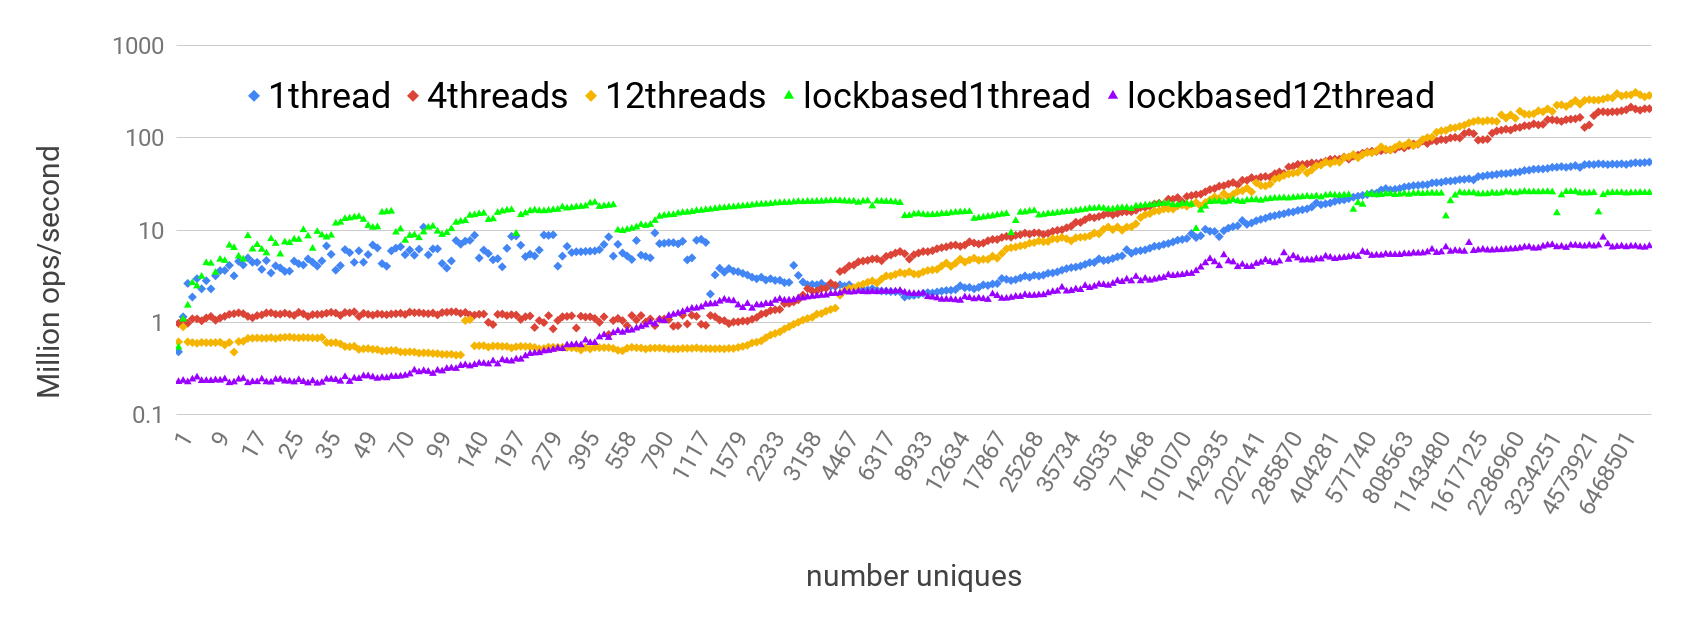
\includegraphics[width=\textwidth]{graphics/fast-concurrent/theta-write-only.png}
\caption{Throughput, loglog scale}
\label{fc-fig:throughput:native}
\end{subfigure}
\begin{subfigure}{\columnwidth}\centering
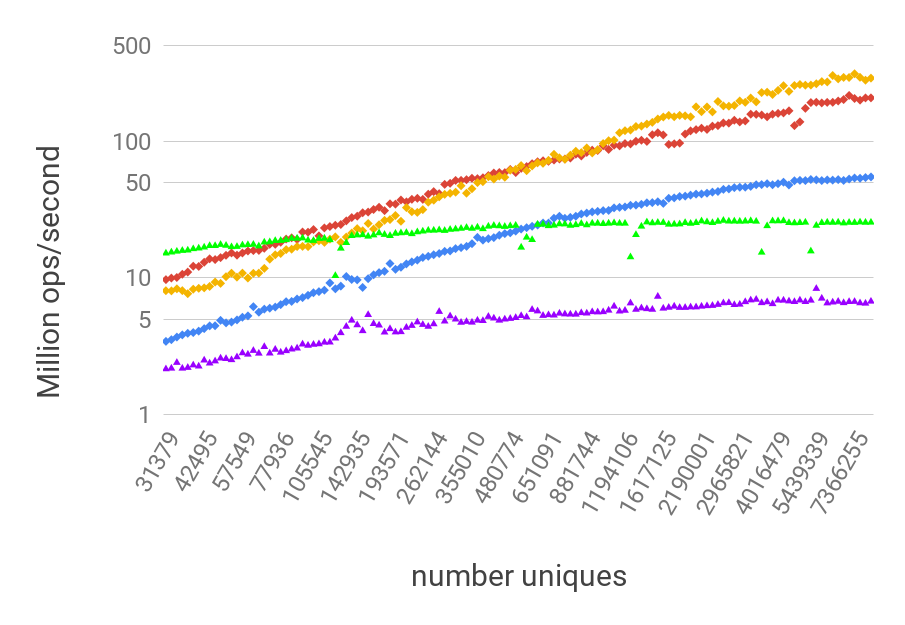
\includegraphics[width=\textwidth]{graphics/fast-concurrent/theta-write-only-zoomin.png}
\caption{Zooming-in on large sketches}
\label{fc-fig:throughput:large}
\end{subfigure}
  \caption{Write-only workload, $k = 4096$, $\epsilon=0.04$.}
  \label{fc-fig:throughput}
\end{figure*}


\paragraph{Mixed workload}
Figure~\ref{fc-fig:mixed-throughput} presents the throughput measurements
of a mixed read-write workload. We compare runs with a single updating thread and $2$
updating threads (and $10$ background reader threads).
Although we see similar trends as in the write-only workload, the effect of
background readers is more pronounced in the lock-based implementation than in the concurrent one;
this is expected as the reader threads compete for the same lock as the writers.
The peak throughput of a single writer thread in the concurrent implementation is $55$M ops/sec both with and
without background readers. The peak throughput of a single writer thread in the lock-based
implementation degrades from $25$M ops/sec without background reads to $23$M ops/sec with them; this is an almost $10$\% slowdown in performance.
Recall that in this scenario reads are infrequent, and so the degradation is not dramatic.

\begin{figure}[tb]
\setlength{\abovecaptionskip}{0pt}
\setlength{\belowcaptionskip}{0pt}
\setlength\textfloatsep{0pt}
	\centering
	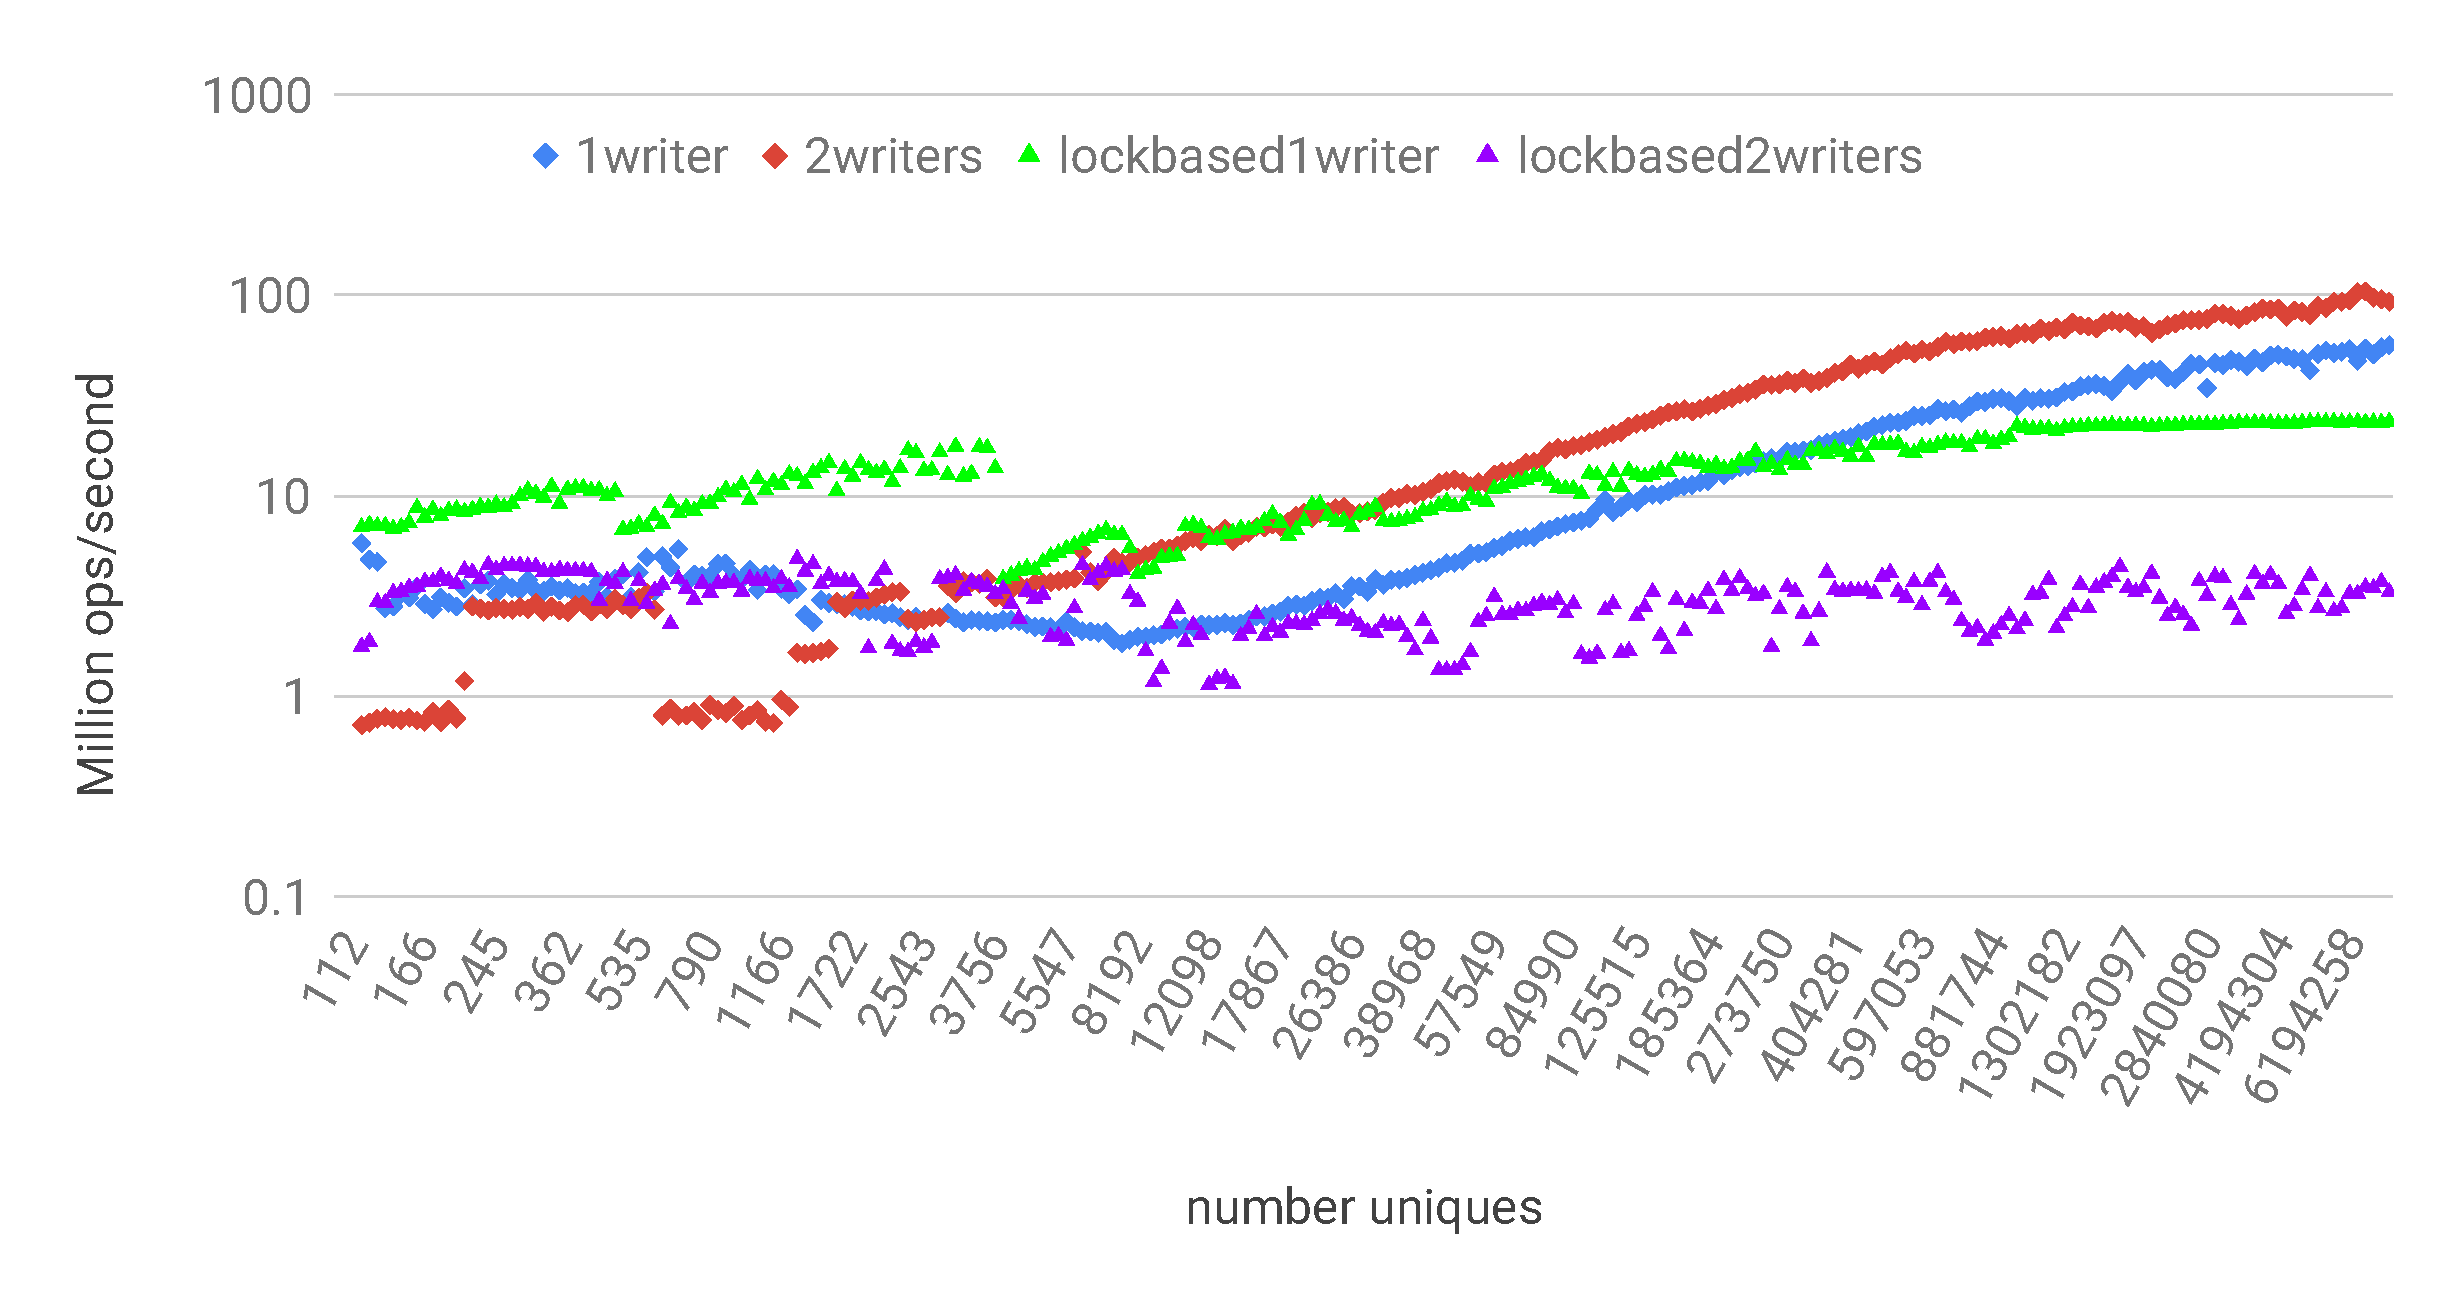
\includegraphics[width=\columnwidth]{graphics/fast-concurrent/theta-mixed.pdf}
	\caption{{Mixed workloads: writers with background reads, $k = 4096$, $\epsilon=0.04$.}}
	\label{fc-fig:mixed-throughput}
\end{figure}


\paragraph{Scalability results}
To provide a better scalability analysis, we aim to maximize the number of threads working on the
sketch. Therefore, we run this test on a larger machine -- we use a 32-core Xeon E5-4650 processors.
We ran an \emph{update-only} workload in which a sketch is built from a very large stream, repeating
each test 16 times.

In Figure~\ref{fc-fig:performance} (in the introduction) we compare the scalability
of our concurrent $\Theta$ sketch and the original sketch wrapped
with a read/write lock in an update-only workload, for $b=1$ and $k=4096$.
As expected, the lock-based sequential sketch does not scale, and
in fact it performs worse when accessed concurrently by many threads.
In contrast, our sketch achieves almost perfect scalability.
$\Theta$ quickly becomes small enough to allow filtering out most of the updates and so the
local buffers fill up slowly.


\subsection{Accuracy-throughput tradeoff}
\label{fc-ssec:tradeoffs}

The speedup achieved by eager propagation in small streams is presented in Figure~\ref{fc-fig:speedup}.
This is an additional advantage of eager propagation in small streams, beyond the accuracy benefit reported in Figure~\ref{fc-fig:accuracy-res}. 
The improvement is as high as $84$x for tiny sketches, and tapers off as the sketch grows.
The slowdown in performance when the sketch size exceeds $2k$ can be explained by the reduction
in the local buffer size (from $b=16$ to $b=5$), needed in order to accommodate for the required error bound.

\begin{figure}[tb]
\setlength{\abovecaptionskip}{0pt}
\setlength{\belowcaptionskip}{0pt}
\setlength\textfloatsep{0pt}
	\centering
	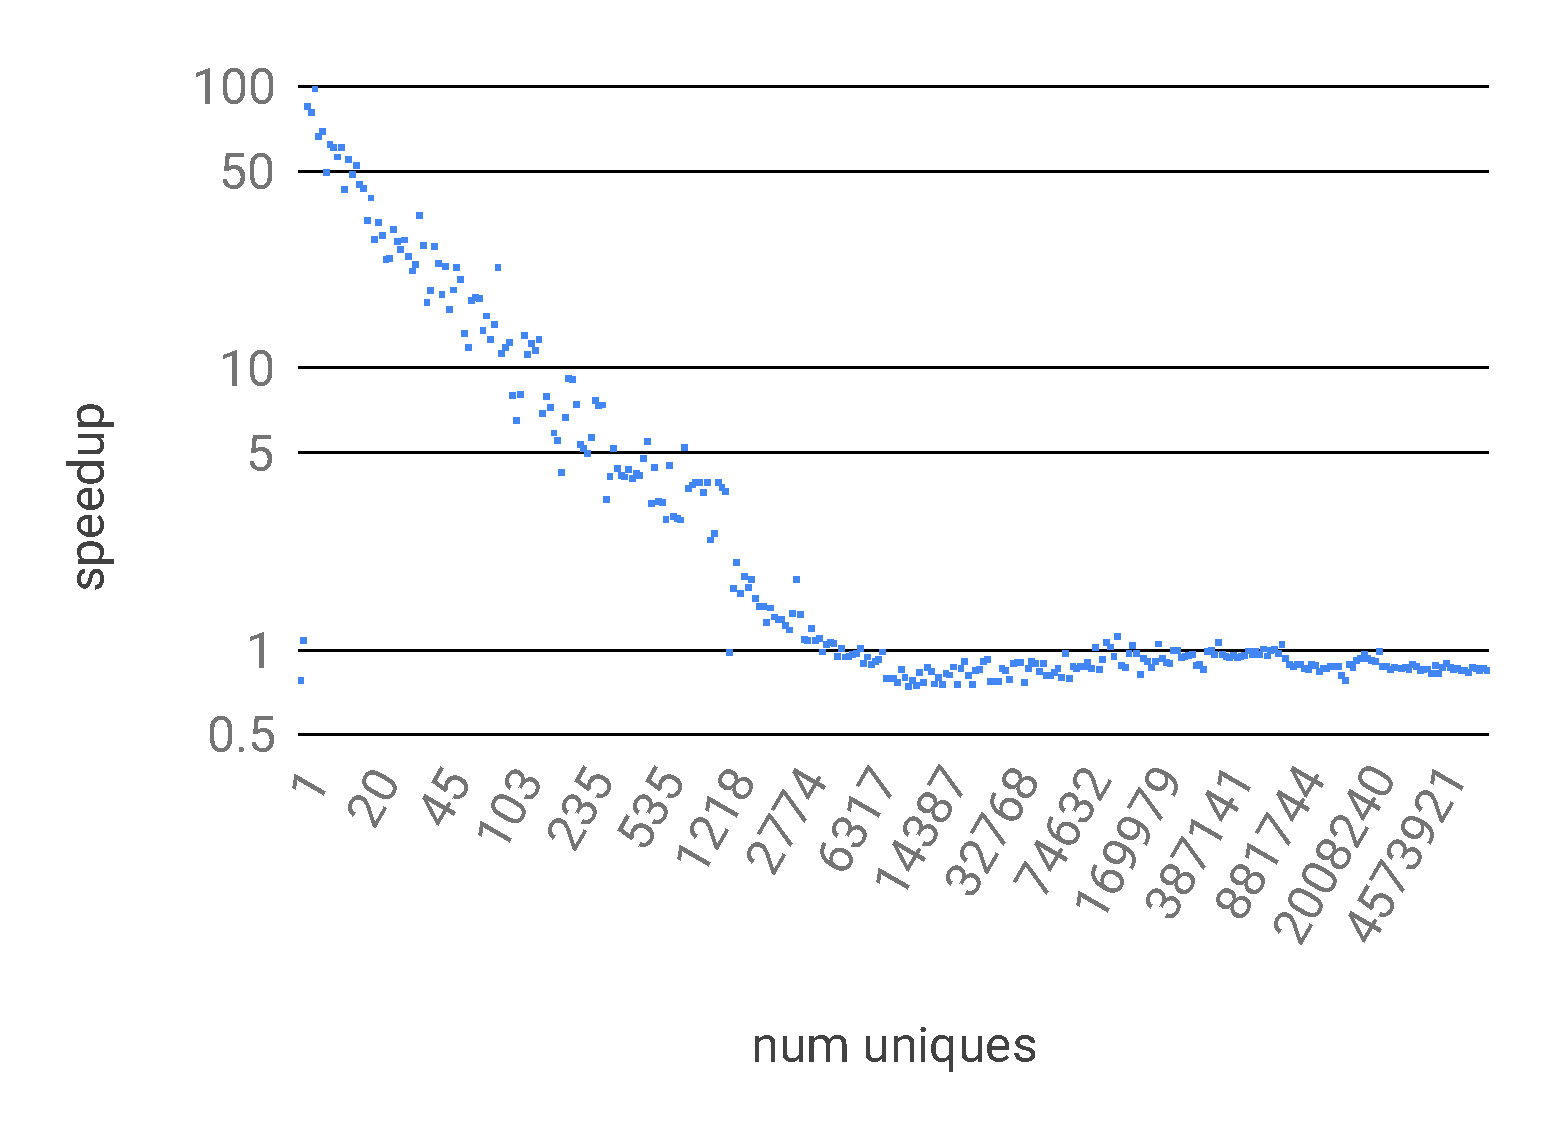
\includegraphics[width=\columnwidth]{graphics/fast-concurrent/eager-speedup.pdf}
	\caption{{Throughput speedup of eager ($\epsilon=0.04$) vs no-eager ($\epsilon=1.0$) propagation, $k = 4096$.}}
	\label{fc-fig:speedup}
\end{figure}


Next we discuss the impact of $k$.
One way to increase the throughput of the concurrent $\Theta$ sketch is by
increasing the size of the global sketch, namely increasing $k$. On the other hand,
this change also increases the error of the estimate.
Table~\ref{fc-tab:tradeoff} presents the tradeoffs between performance and accuracy.
Specifically, it presents the crossing-point, namely the smallest stream size for which the concurrent
implementation outperforms the lock-based implementation (both running a single thread). It further presents
the maximum values (across all stream sizes) of the median error and 99th percentile error for a variety of $k$ values.
The table shows that as the sketch promises a smaller error (by using a larger $k$), a larger stream size is needed to justify using
the concurrent sketch with all its overhead.

\begin{table}[htb]
\center{\small{
\begin{tabular}{lrrr}
\hline 
& thpt crossing point & mean error & error $Q=0.99$ \\
\hline 
$k=256$ &  15,000 &	0.16 & 0.27 \\
\hline 
$k=1024$ &  100,000 &	0.05 & 0.13 \\
\hline 
$k=4096$ & 700,000	& 0.03	& 0.05	\\ 
\hline 
\end{tabular}
}}
\caption{{Performance vs accuracy as a function of $k$.}}
\label{fc-tab:tradeoff}
\end{table}  




%\input{sections/appendixEvaluation.tex}
%\input{sections/Evaluation.tex}


\section{Conclusions}
\label{fc-sec:discussion}

Sketches are widely used by a range of applications
to process massive data streams and answer queries about them.
Library functions producing sketches
are optimized to be extremely fast, often digesting tens of millions of stream elements per second. 
We presented a generic algorithm for parallelizing such sketches and serving
queries in real-time; the algorithm is strongly linearizable with regards to relaxed semantics.
%\inred{We discussed the necessity of adapation for small streams, and how to implement such an adapation.}
We showed that the error bounds of two representative sketches,
$\Theta$ and Quantiles, do not increase drastically with such a relaxation. We also
implemented and evaluated the solution, showed it to be scalable {and accurate}, and integrated it into
the open-source Apache DataSketches library. While we analyzed only two sketches, future work
may leverage our framework for other sketches. Furthermore, it would be interesting to investigate
additional uses of the hint, for example, in order to dynamically adapt the size of the local buffers
and respective relaxation error.